
% ---------------------------------------------------
%
% Trabajo de Fin de Grado. 
% Author: Alejandro Hernández Padrón. 
% Capítulo: La aplicación ULL-AR. 
% Fichero: Cap4_TheApplication.tex
%
% ----------------------------------------------------
%


\lstset{stringstyle=\color{purple}}
\chapter{La aplicación ULL-AR} \label{chap:LaAplicacion} 

En este capítulo explicaremos la aplicación ULL-AR utilizando la especificación de requisitos de esta y explicando su funcionamiento.

\section{Requisitos y ventanas de la aplicación} % (fold)

Nos dispondremos a exponer los requisitos de la presente aplicación propuesta para el desarrollo de este TFG.

Se trata de una aplicación para móviles, más concretamente, a aquellos dispositivos que utilizan Android como sistema operativo. Es una aplicación diseñada para los estudiantes de la Universidad de La Laguna, la cual les permita ubicarse, detectar y reconocer las instalaciones y edificios pertenecientes a la universidad, mediante técnicas de realidad aumentada basadas en la geolocalización.

Los requisitos principales de la aplicación son:
\begin{itemize}
    \item La aplicación se desarrollará para dispositivos con Android. Se utilizará Android Studio como IDE para su desarrollo.
    \item Se implementarán técnicas de realidad aumentada basadas en la geolocalización para mostrar al usuario la instalación de la ULL a la cual apunte con la cámara.
    \item Las instalaciones, junto a su información correspondiente, estarán ubicadas en un base datos en la nube. El servidor que se conecte con esta base de datos también deberá estar en la nube.
\end{itemize}

\subsection{Especificación detallada de los requisitos} 

La aplicación se iniciará una Splash Screen \cite{URL::SplashScreen} o pantalla de inicio con el logo de la Universidad de La Laguna. Esta pantalla dará paso a una ventana de login.

Para poder utilizar la aplicación, el usuario ha de ser alumno de la Universidad de La Laguna y poseer su respectiva cuenta de Google con el correo institucional de la ULL. Este correo ha de tener el siguiente formato: ``\textit{aluxxxxxxxxxx@ull.edu.es}''. Sin ella no se podrá acceder a la aplicación. Además, se podrá cerrar la sesión de esta cuenta.

Una vez logueado accederemos a una ventana de \textit{Inicio} en la que aparecerá un acceso directo a las ventanas de \textit{Mapa ULL} y \textit{Navegación en modo RA} que explicaremos más adelante. A su vez, dispondrá de los accesos directos a enlaces de interés de Universidad de La Laguna que se abrirán en un navegador externo. 

Una vez dentro de la aplicación, tendremos un menú para movernos por las diferentes ventanas. Se utilizará un menú deslizante lateral o \textit{Navigation Drawer} \cite{URL::NavigationDraw} ubicado en la parte superior izquierda de la aplicación. Este menú deberá ser simple e intuitivo.

Como accesos en este menú disponemos de las siguientes ventanas:

\begin{itemize}
    \item Inicio. Ventana inicial con la que se abre la aplicación.
    \item Mapa ULL. Esta ventana contendrá un mapa de la universidad con todas las instalaciones en la base de datos. 
    \item Navegación en modo RA. En esta ventana, mediante el uso de la cámara, se identificarán las instalaciones universitarias a los que el usuario apunte y permitirá mostrar una pestaña con información detallada de las mismas.
    \item instalaciones de la ULL. Contiene todas la ubicaciones e instalaciones de la Universidad de La Laguna y permitirá la búsqueda de estas. 
    \item Configuración. Permitirá acceder a los ajustes de la aplicación.
    \item Cerrar cesión. Cerrará la sesión actual y nos devolverá a la ventana de login.
    \item Info. Información de aplicación así como de su autor.
\end{itemize}

Una instalación de la ULL corresonde a un centro, edificio, facultad, instituto, polideportivo, etc. Cada instalación de la universidad tendrá una ficha de información que será accesible desde una ventana de la aplicación con la siguiente información:

\begin{itemize}
    \item \textbf{Id}: campo para identificar la instalación.
    \item \textbf{Nombre}: nombre oficial de la instalación.
    \item \textbf{Ubicación}: la ubicación exacta en la que se encuentra la instalación. 
    \item \textbf{Descripción}: descripción de la instalación con el objetivo y actividades que se desarrollan en él.
    \item \textbf{Imagen}: imagen de la instalación.
    \item \textbf{Lista de enlaces de interés}: una lista con los enlaces a las instituciones, servicios, departamentos y grados que se imparten en esta instalación.
\end{itemize}

Esta información estará guardada en una base de datos en la nube. Para acceder a esta, se dispondrá de un servidor en la nube que conecte con la base de datos y envié la información a la aplicación.

\subsection{Ventanas de la aplicación}

Nada más iniciar la aplicación nos encontramos con dos ventanas.

\begin{figure}[h]
\hspace*{\fill}%
\begin{subfigure}[h]{0.32\linewidth}

\includegraphics[width=\linewidth]{splashApp}
\caption{Splash-Screen.}
\label{fig:splashApp}
\end{subfigure}
\hfill%
\begin{subfigure}[h]{0.32\linewidth}
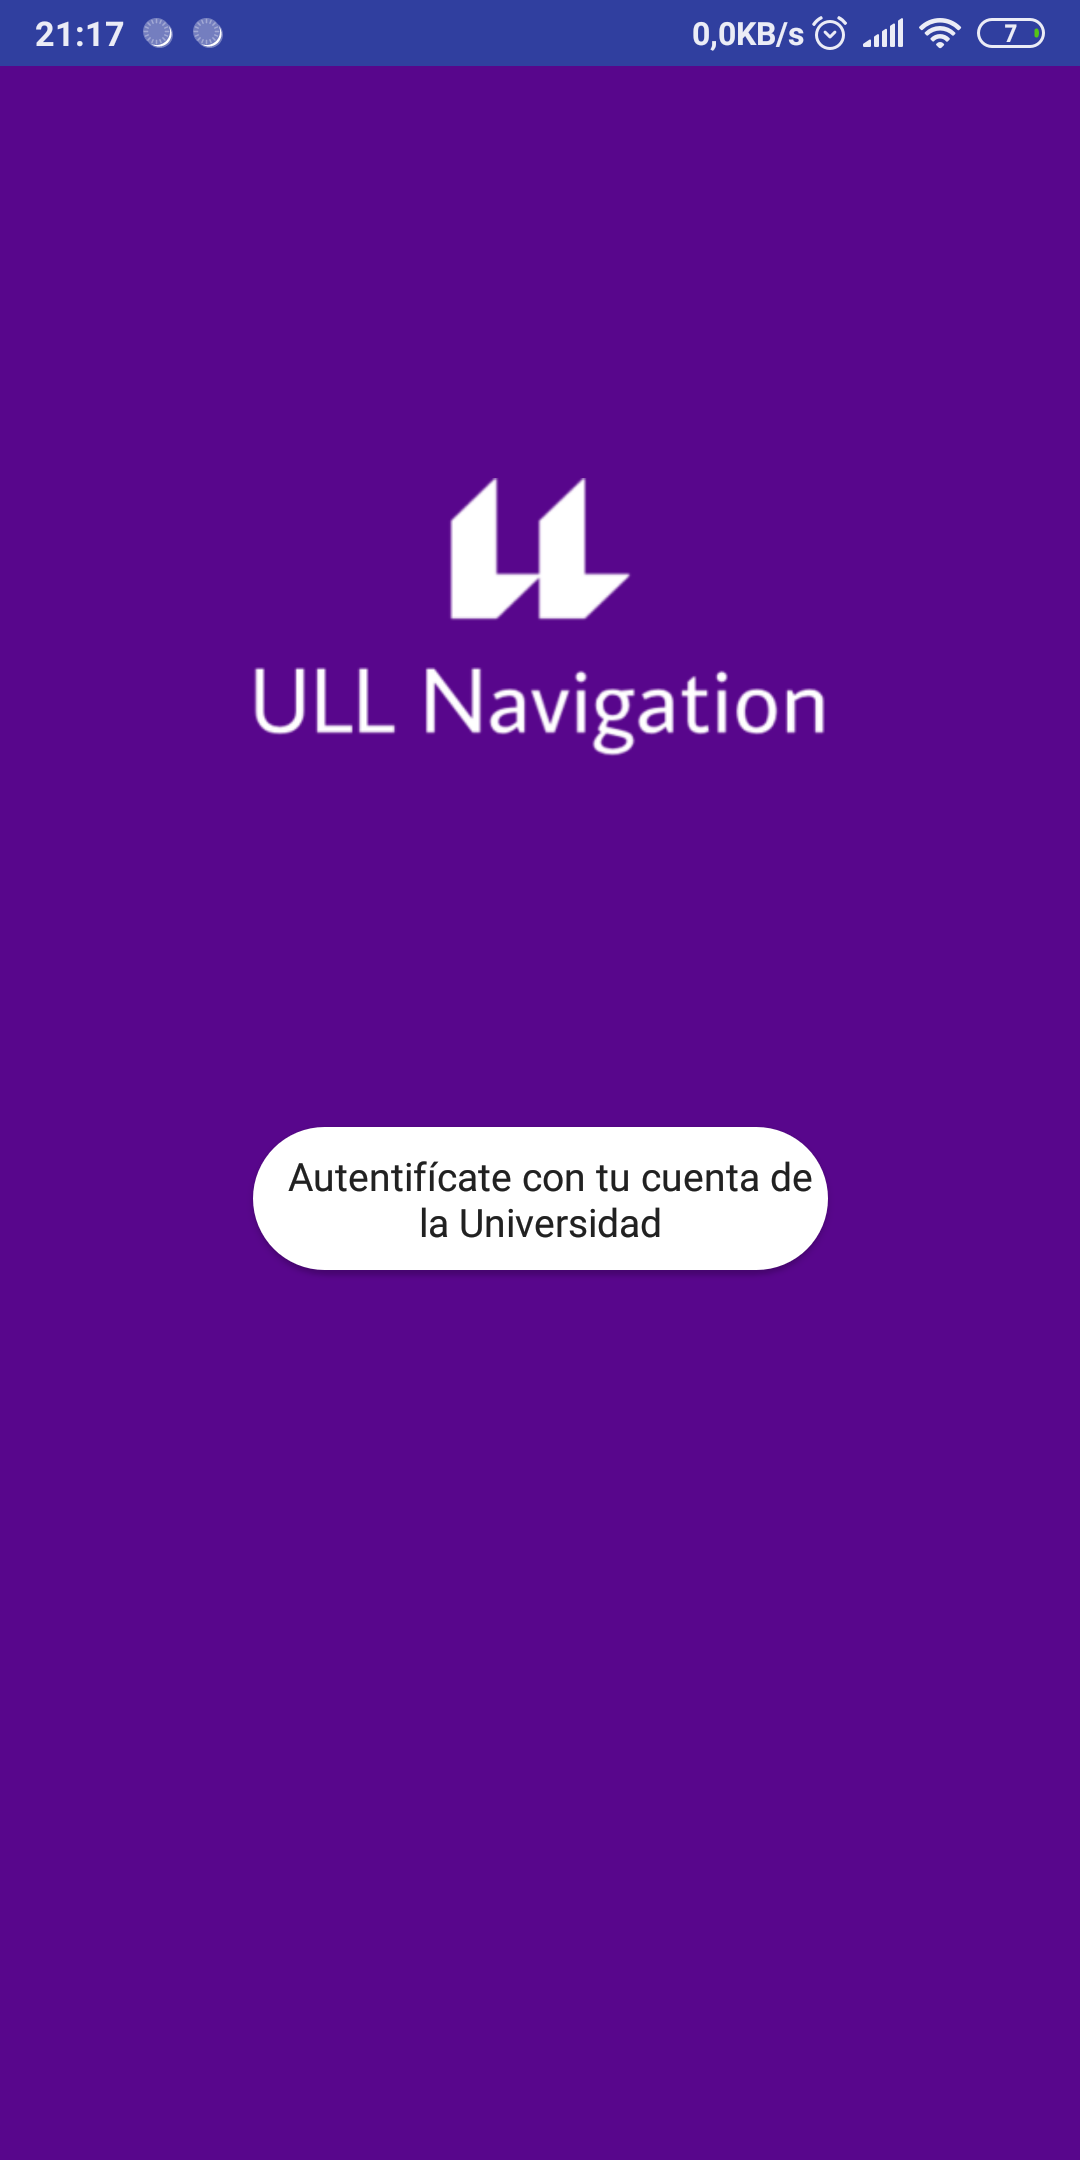
\includegraphics[width=\linewidth]{loginApp}
\caption{Login.}
\label{fig:loginApp} 
\end{subfigure}%
\caption{Ventanas de iniciales de \textit{ULL-AR}.}
\hspace*{\fill}%
\end{figure}
  
La primera ventana (véase Figura \ref{fig:splashApp}) es la pantalla de inicio o Splash Screen que aparece cuando ejecutamos la aplicación. Tras unos segundos, se carga la ventana de \textit{Login} (véase Figura \ref{fig:loginApp}). Para poder loguearnos deberemos tener una cuenta de Google de la ULL. Una vez que presionamos en el botón del medio, se nos abrirá una ventana de diálogo para que pongamos nuestra cuenta.

Cuando nos hayamos logueado con éxito, se nos abrirá la venta de \textit{Inicio} (véase Figura \ref{fig:homeApp}). En esta tendremos una lista de accesos directos a las funcionalidades principales de la aplicación, como son \textit{Navegación en modo RA}, \textit{Mapa ULL} y una serie de enlaces a sitios web relacionados con la ULL.

\begin{figure}[h]
    \hspace*{\fill}%
    \begin{subfigure}[h]{0.35\linewidth}
    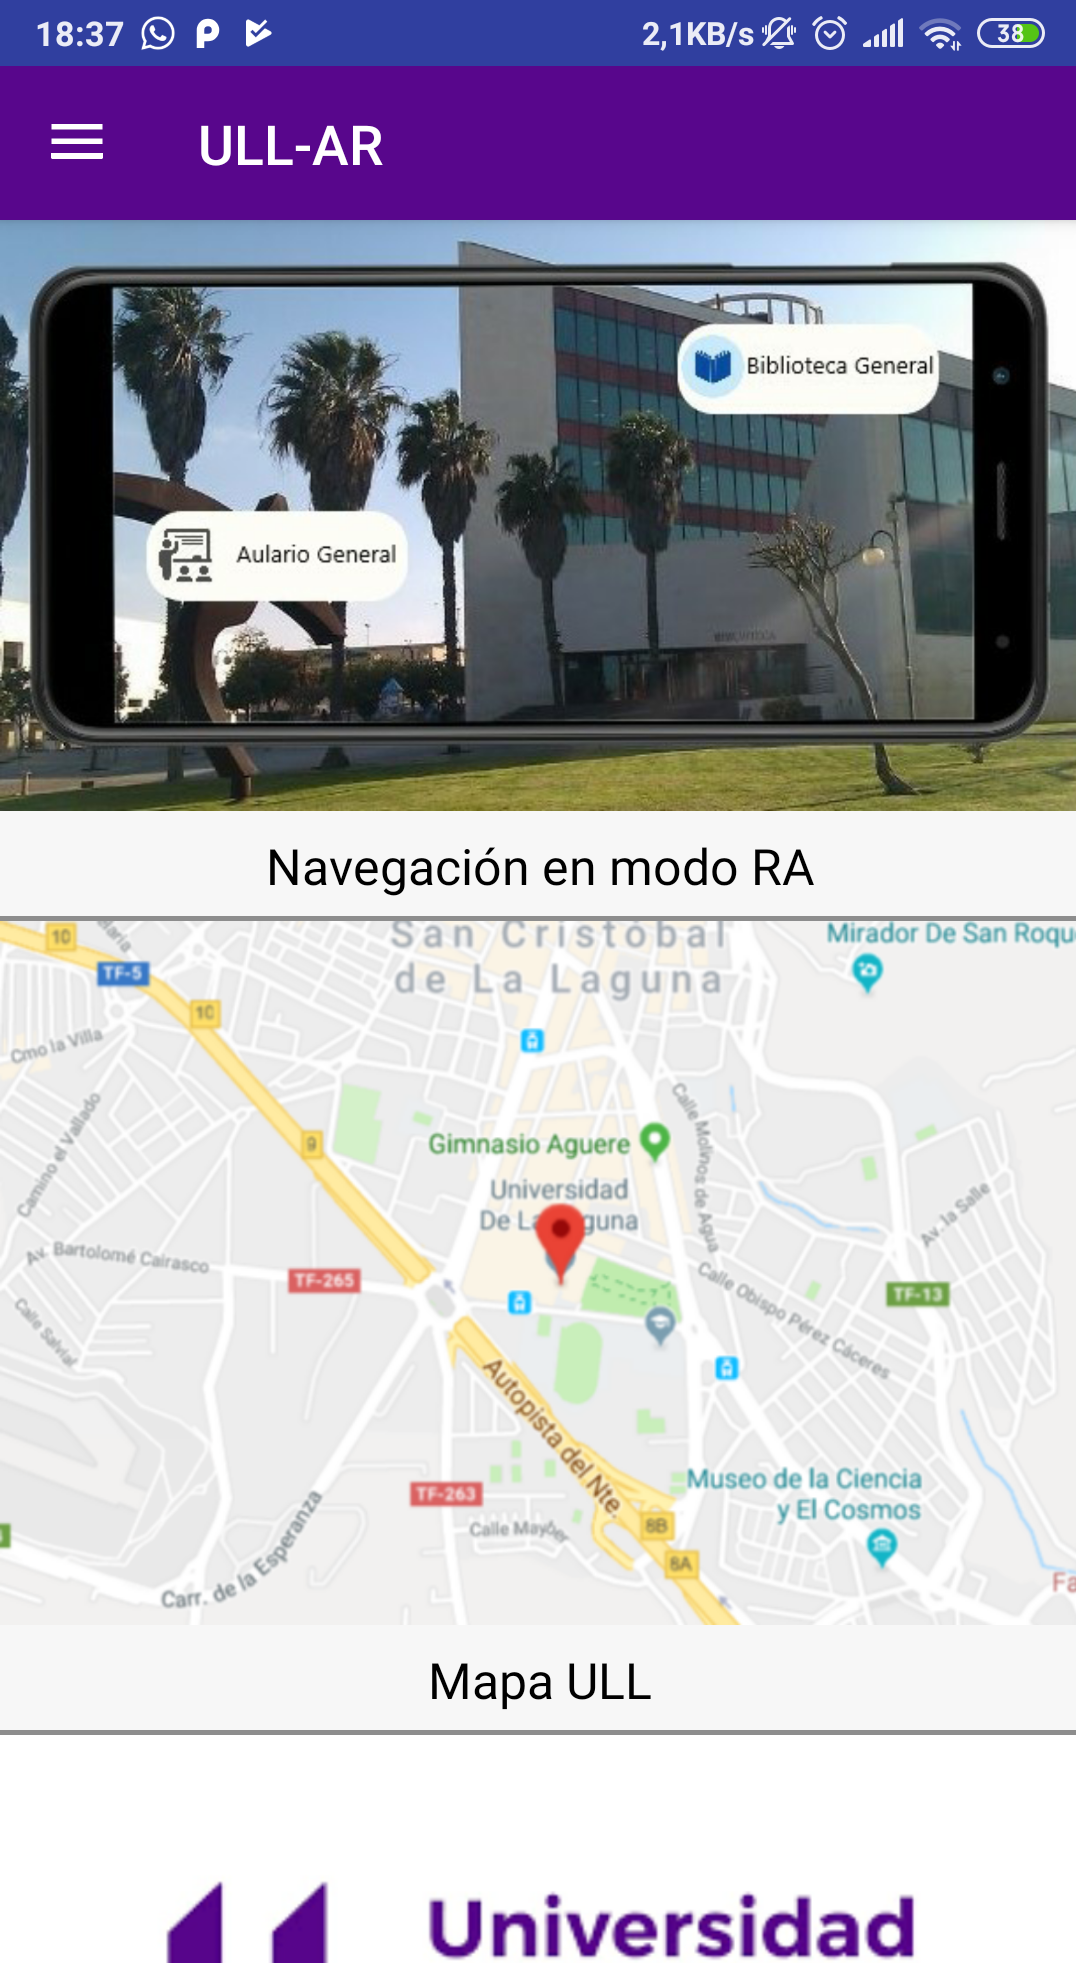
\includegraphics[width=\linewidth]{homeApp}
    \caption{Inicio.}
    \label{fig:homeApp}
    \end{subfigure}
    \hfill%
    \begin{subfigure}[h]{0.35\linewidth}
    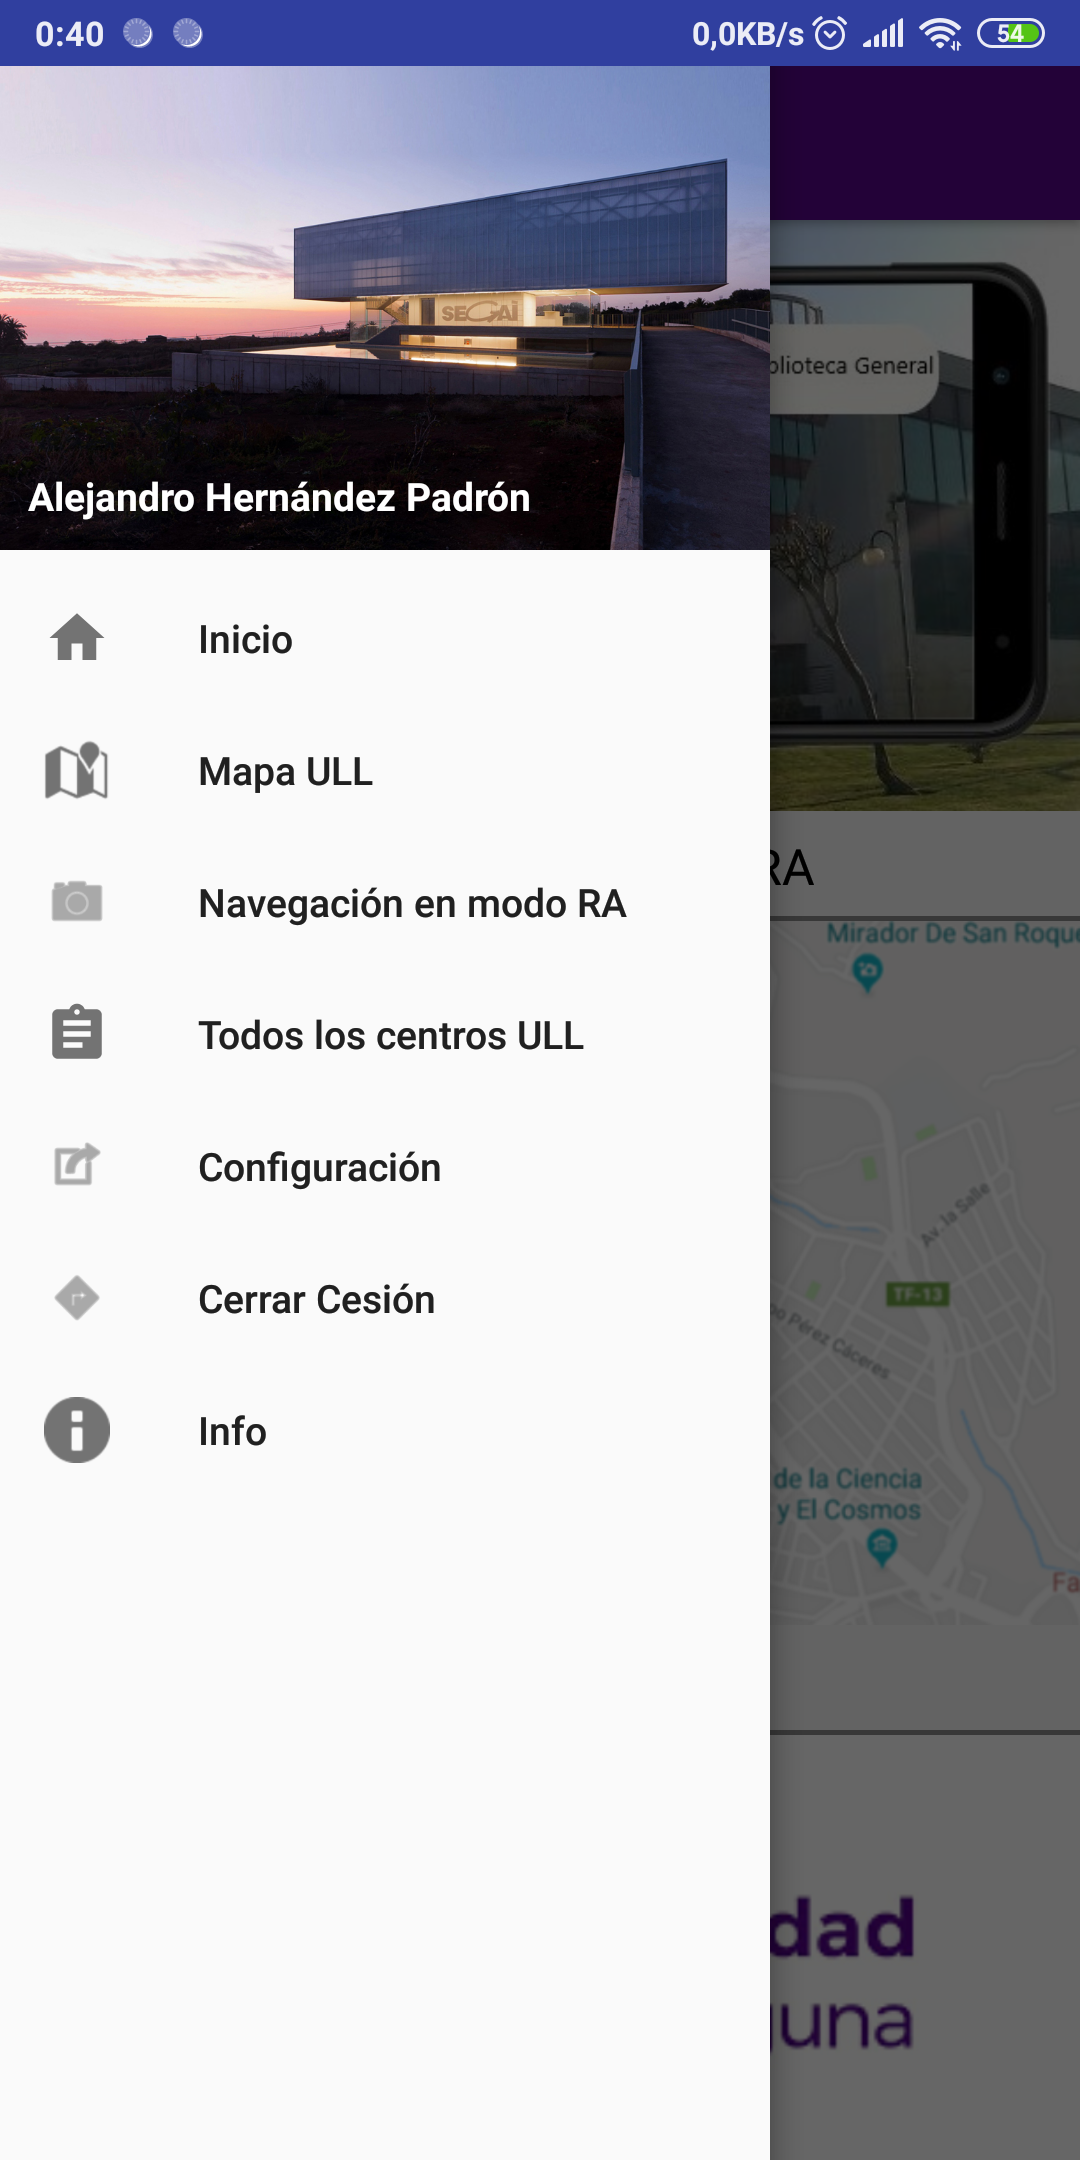
\includegraphics[width=\linewidth]{menuApp}
    \caption{Menu. Navigation Drawer.}
    \label{fig:menuApp}
    \end{subfigure}%
    \caption{Ventana \textit{Inicio} y el \textit{Menú} de \textit{ULL-AR}.}
    \hspace*{\fill}%
\end{figure}

En la esquina superior izquierda de aplicación tenemos el acceso al menú \textit{Navigation Drawer}. Si lo pulsamos se nos desplegará el menú que nos permite movernos por las distintas ventanas de la aplicación (véase Figura \ref{fig:menuApp}).

Si nos movemos a la ventana de \textit{Mapa ULL} (véase Figura \ref{fig:mapsApp}) veremos el mapa de la API de Google Maps. En este mapa nos aparecerán en pines azules las ubicaciones con sus respectivos nombres de la ULL que están guardadas en la base de datos. Cuando el GPS del dispositivo encuentre la ubicación aparecerá un pin rojo que indicará nuestra posición. En la parte de abajo en el centro disponemos de un botón llamado ``AR Mode'' que nos llevará directo a la ventana de \textit{Navegación en modo RA}.
  
\begin{figure}[h]
    \centering
    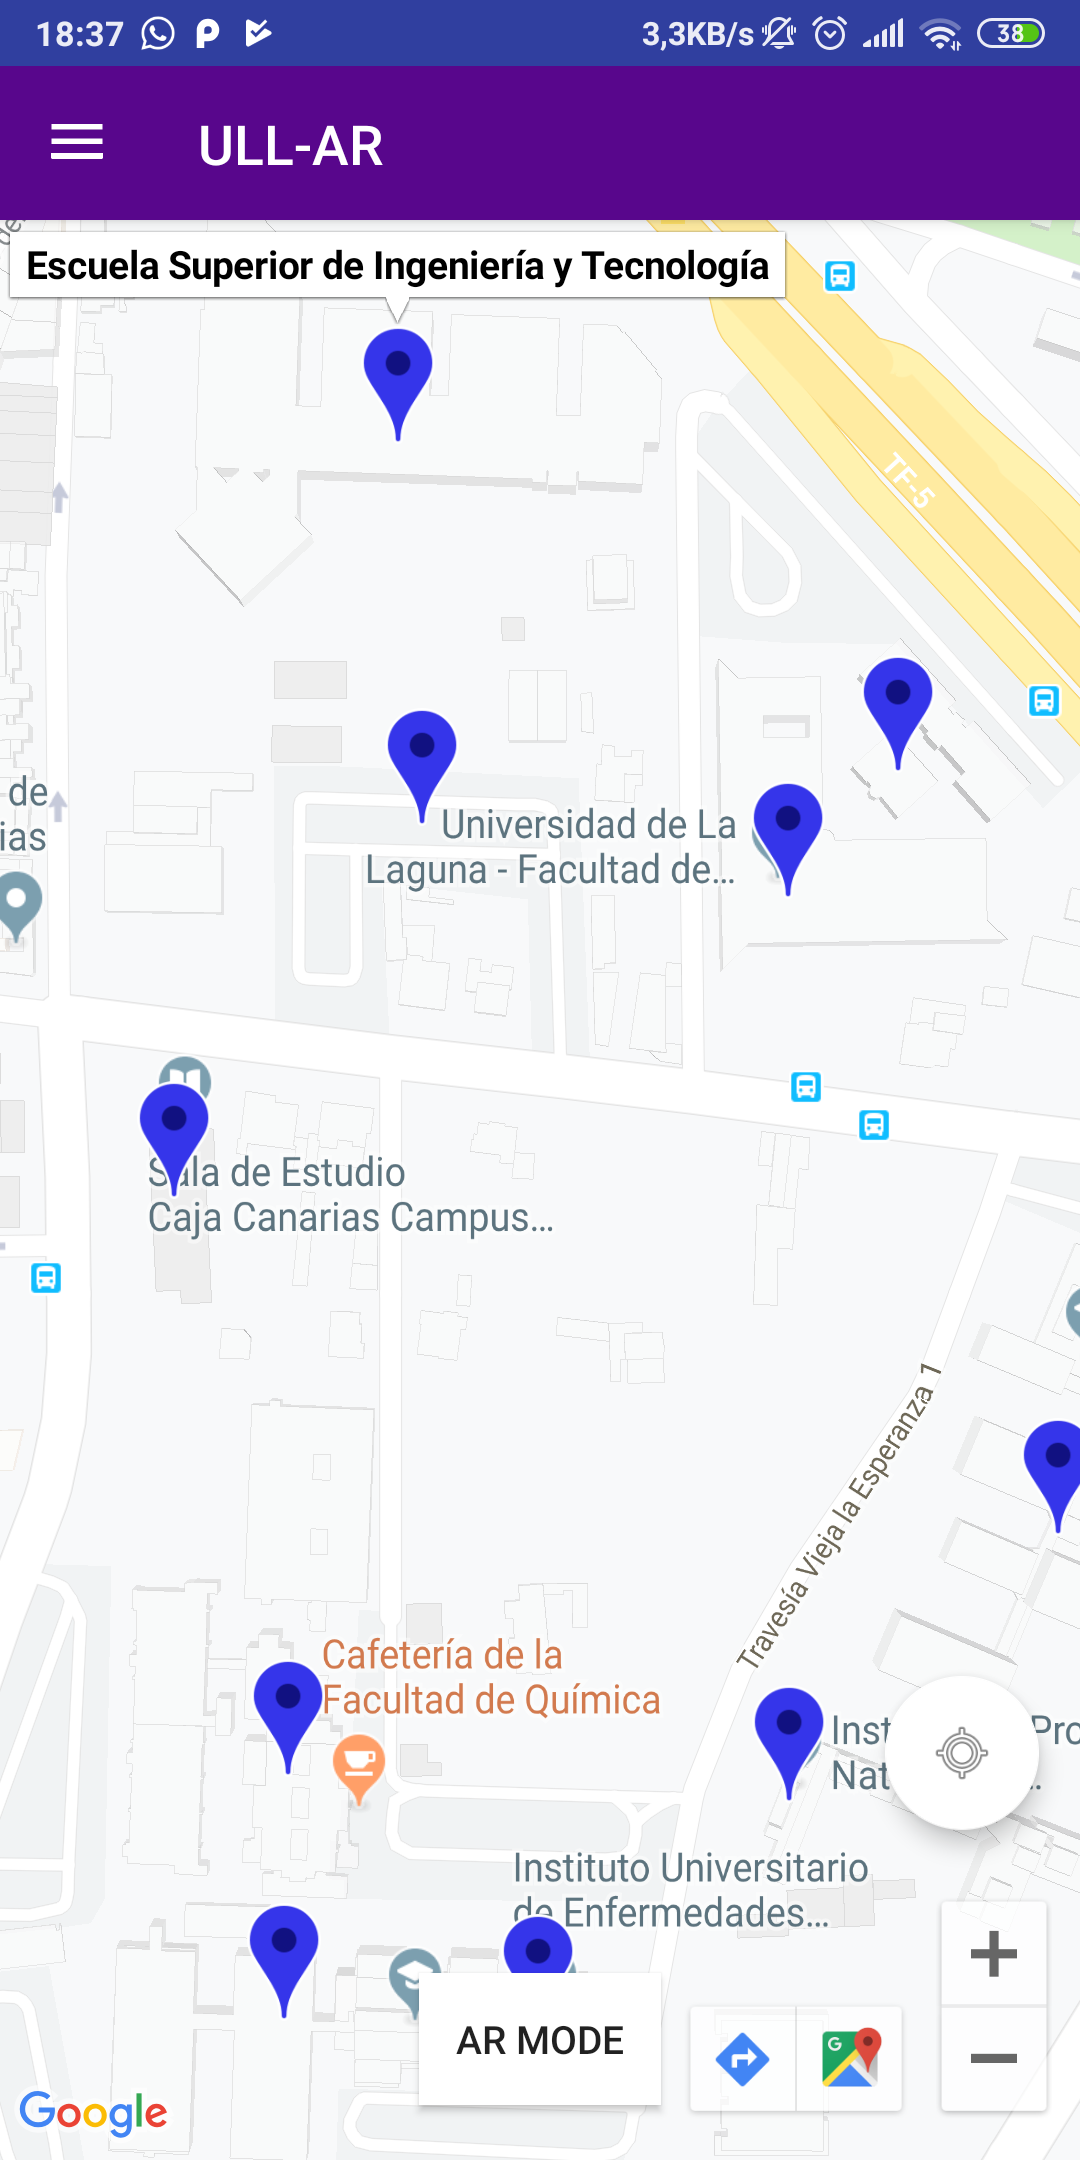
\includegraphics[width=0.38\linewidth]{mapsApp}
    \caption{Mapa ULL.}
    \label{fig:mapsApp}
\end{figure}

En la ventana de \textit{Navegación en modo RA} se nos mostrará la imagen obtenidad de la cámara del dispositivo, con ella el usuario podrá ver en la pantalla la instalación a la que se apunte. Encima de esta imagen se mostrará un texto en el que nos aparecerán dos mensajes: uno para indicar a usuario que apunte a alguna instalación de la ULL, y una vez que se el usuario se encuentre apuntando a una instalación, el mensaje anterior se cambiará por el nombre de la instalación y, al mismo tiempo, aparecerá un pequeño boton debajo del texto que nos llevará a la ventana de \textit{Información de la instalación} (véase Figura \ref{fig:siteInfoApp}), con la información de la instalación. Por último en la parte de abajo se nos mostrará un botón que nos indicará si se han encontrado más instalaciones a parte de la que se nos muestra en la parte de arriba. Esté botón nos llevará a una ventana con una lista de estas instalaciones.



% \begin{figure}[h]
%     \hspace*{\fill}%
%     \begin{subfigure}[h]{0.35\linewidth}
%     \includegraphics[width=\linewidth]{App}
%     \caption{Ventana de \textit{Inicio}}
%     \label{fig:homeApp}
%     \end{subfigure}
%     \hfill%
%     \begin{subfigure}[h]{0.35\linewidth}
%     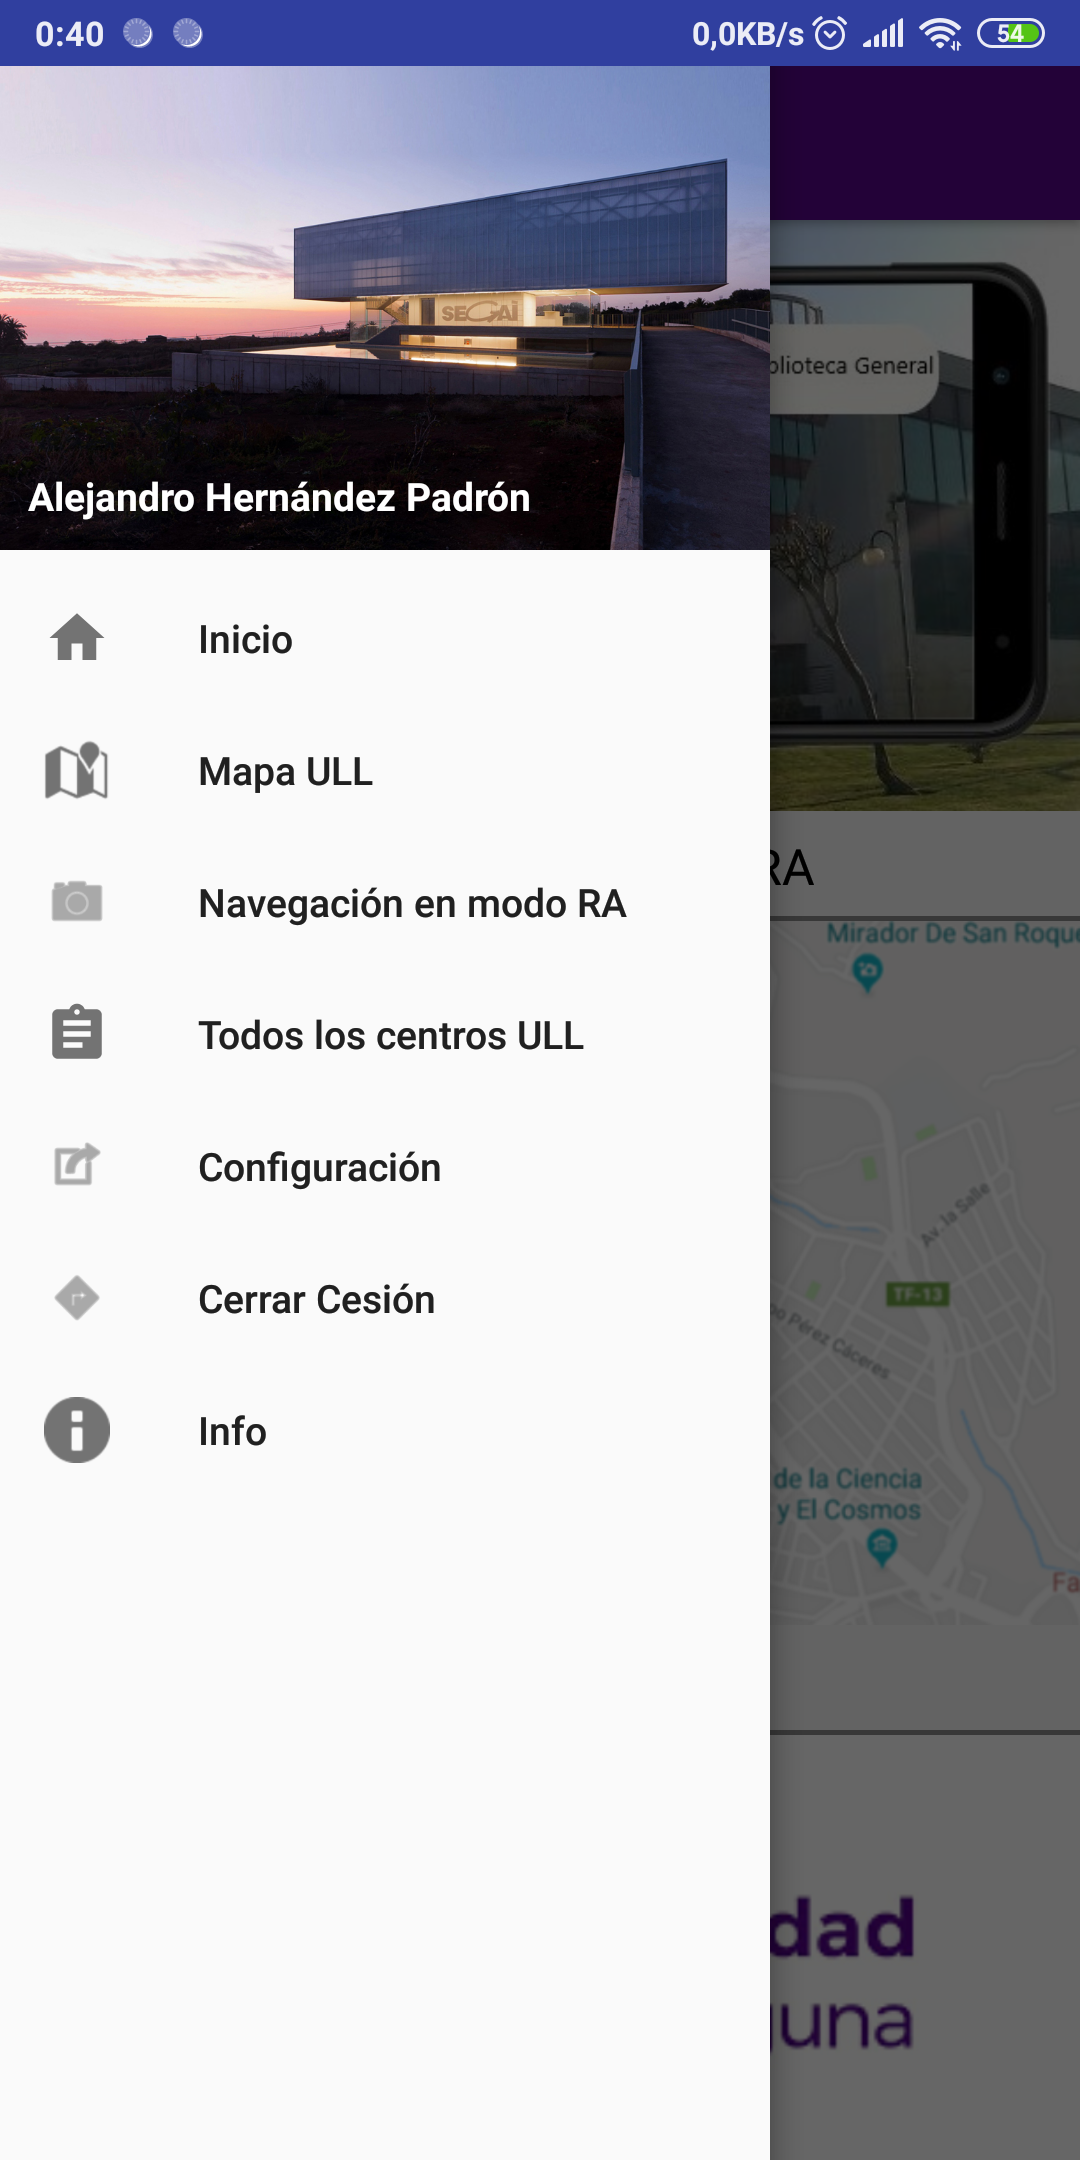
\includegraphics[width=\linewidth]{menuApp}
%     \caption{Ventana de \textit{Inicio}}
%     \label{fig:menuApp}
%     \end{subfigure}%
%     \caption{Ventana Inicio y menú de \textit{ULL-AR}}
%     \hspace*{\fill}%
% \end{figure}

A través del menú de la aplicación podemos acceder a la ventana de \textit{Todas las instalaciones ULL} (véase Figura \ref{fig:allSitesApp}). Aquí se nos mostrarán todas las instalaciones de la ULL que se encuentran en la base de datos. Se podrá hacer una búsqueda de cualquier instalación en la barra superior de la aplicación. Si pulsamos cualquiera de estas instalaciones se nos desplegará una ventana con la información detallada de la instalación.

En la ventana \textit{Información de la instalación} (véase Figura \ref{fig:siteInfoApp}) se dispondrá la información de esta. Aquí se nos mostrará una imagen de este, nombre y descripción de la instalación y una lista de enlaces con los servicios, secretarias, grados y departamentos que podemos encontrar. Disponemos de un botón en la parte inferior de la imagen de la instalación que nos abrirá la ruta a su ubicación en la aplicación de Google Maps para poder llegar a ella.  
 
\begin{figure}[h]
    \hspace*{\fill}%
    \begin{subfigure}[h]{0.35\linewidth}
    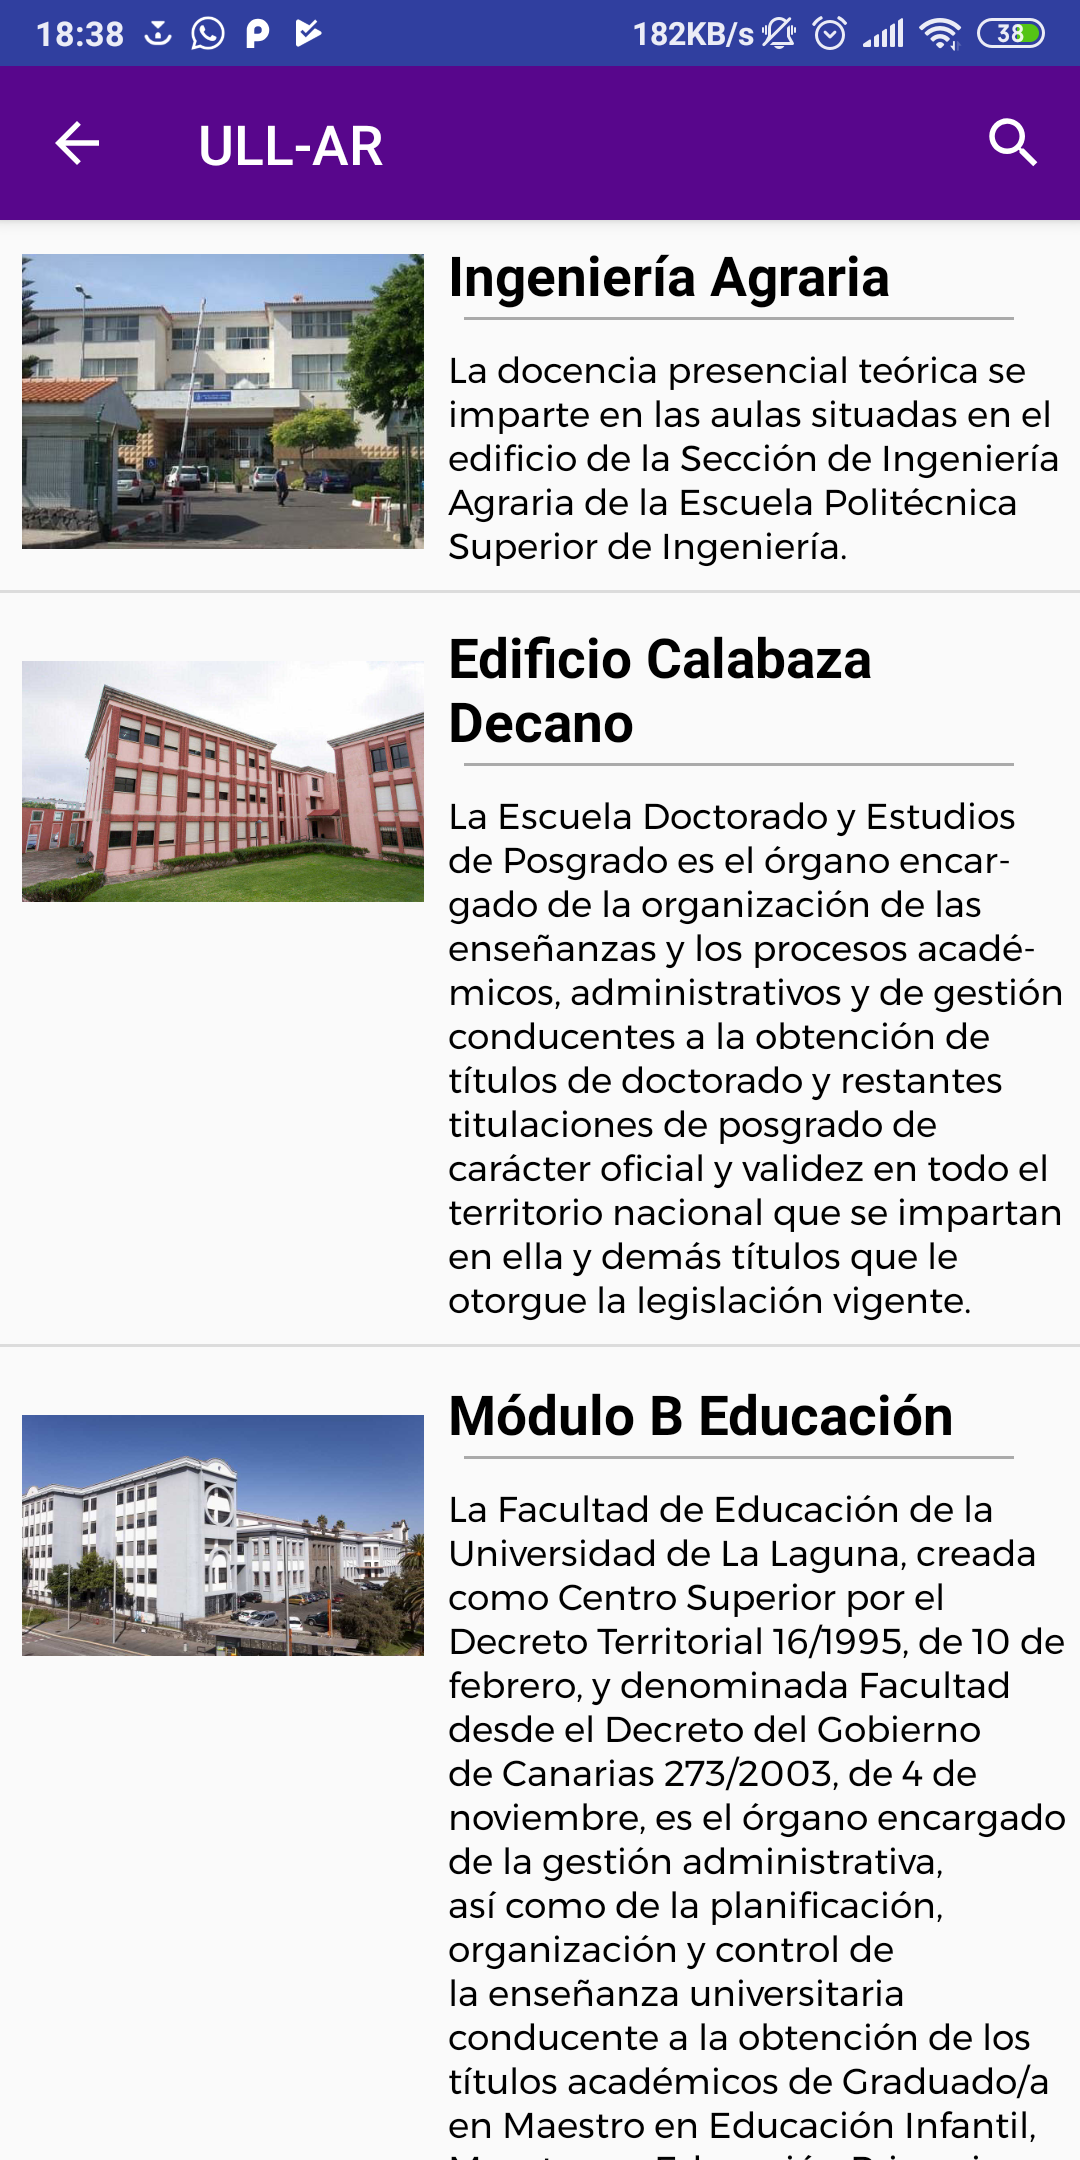
\includegraphics[width=\linewidth]{allSitesApp}
    \caption{Todas las instalaciones ULL.}
    \label{fig:allSitesApp}
    \end{subfigure}
    \hfill%
    \begin{subfigure}[h]{0.35\linewidth}
    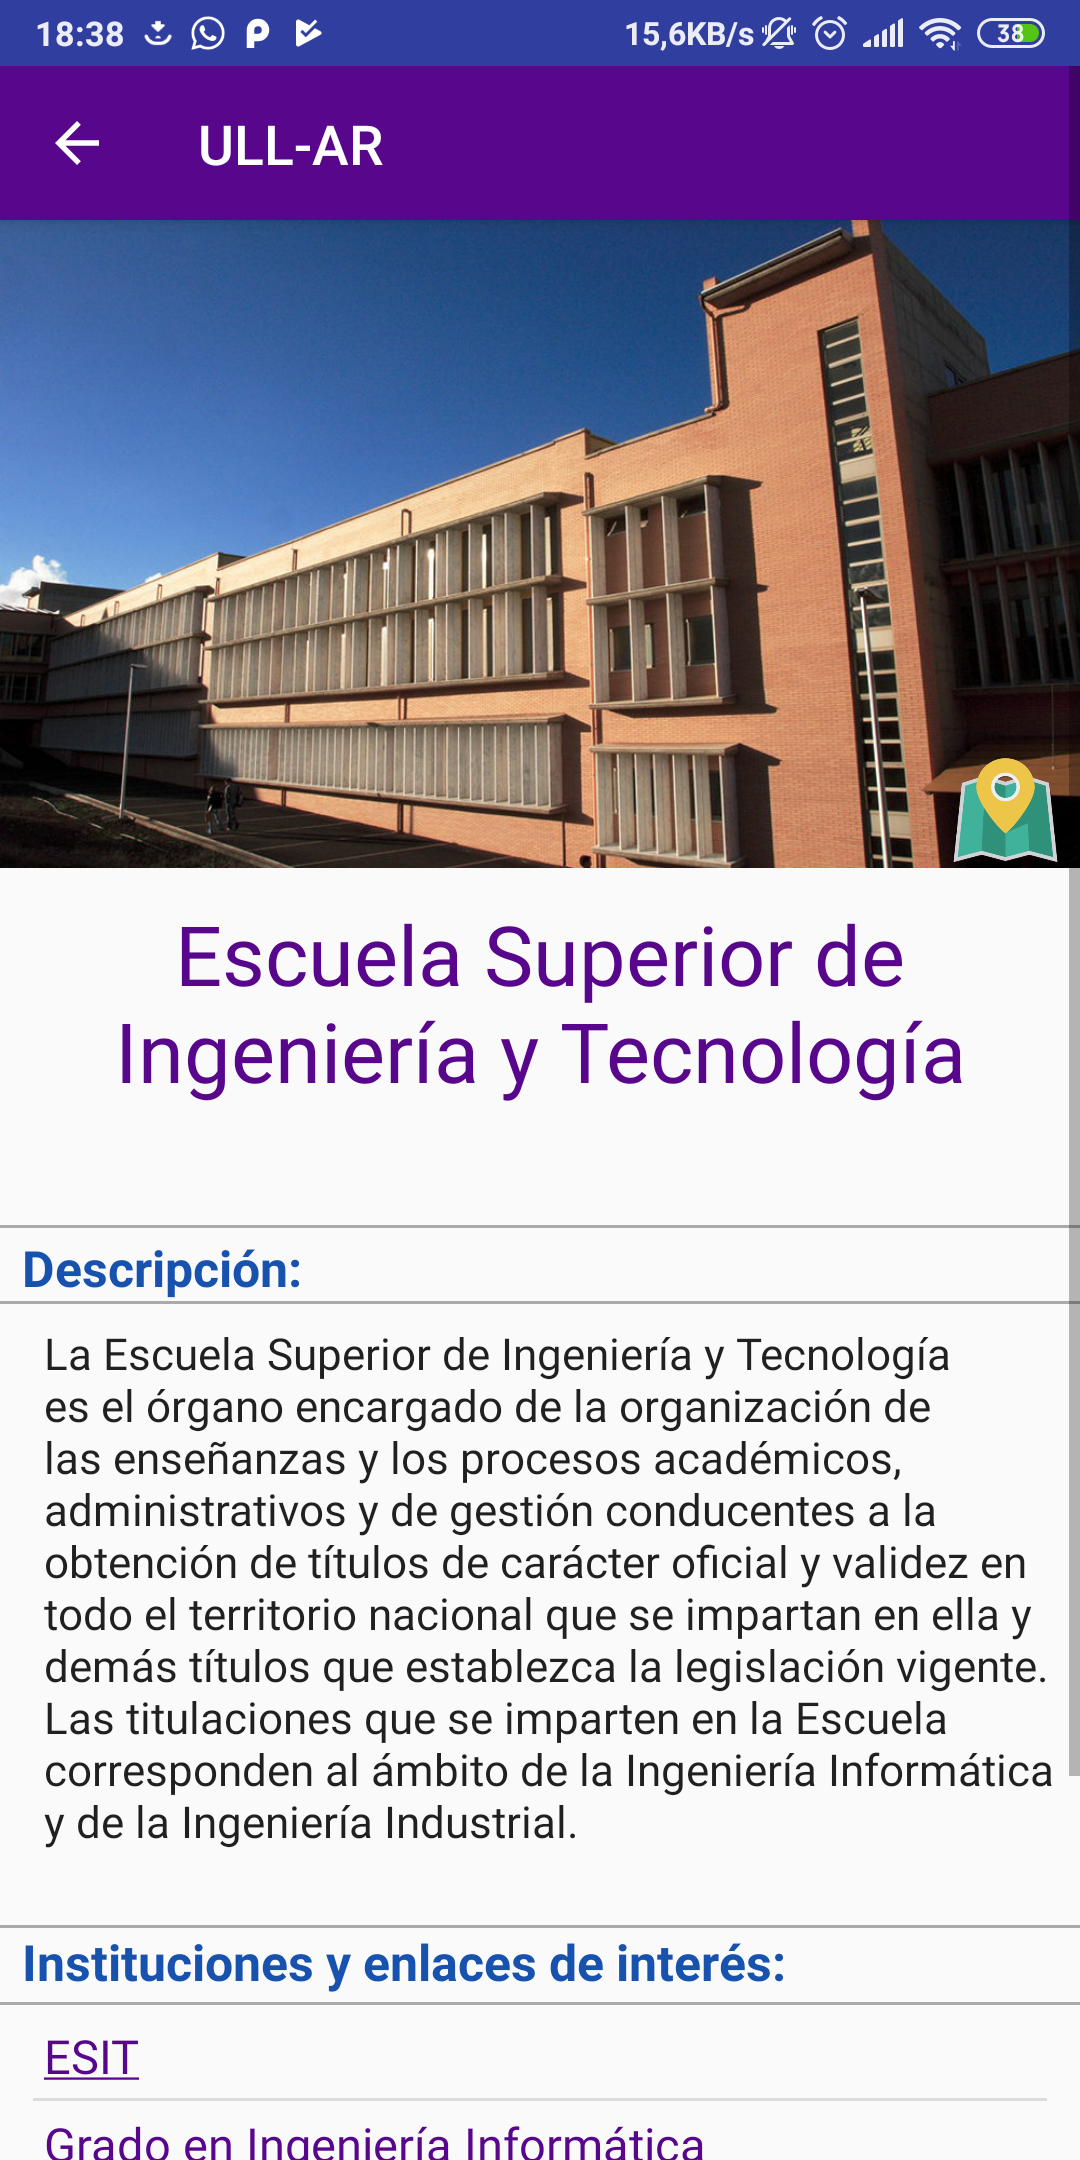
\includegraphics[width=\linewidth]{siteInfoApp}
    \caption{Información de la instalación.}
    \label{fig:siteInfoApp}
    \end{subfigure}%
    \caption{Ventanas de \textit{Todas las instalaciones ULL} e \textit{Información de la instalación} de \textit{ULL-AR}.}
    \hspace*{\fill}%
\end{figure}
 

% \vskip 0.9in

Por último desde el menú podemos acceder a las ventanas de \textit{Configuración} e \textit{Información}.

En la ventana de \textit{Configuración} (véase Figura \ref{fig:settingsApp}) van los ajustes de la aplicación. En ella tenemos la opción para poder configurar si queremos encontrar las instalaciones que se encuentran en el área entre dos circunferencias.

La ventana \textit{Info} (véase Figura \ref{fig:infoApp}) nos muestra información básica de la aplicación como el nombre, versión, correo de contacto, autor y objetivo e información del desarrollo de la aplicación \textit{ULL-AR}. 

\begin{figure}[h]
    \hspace*{\fill}%
    \begin{subfigure}[h]{0.35\linewidth}
    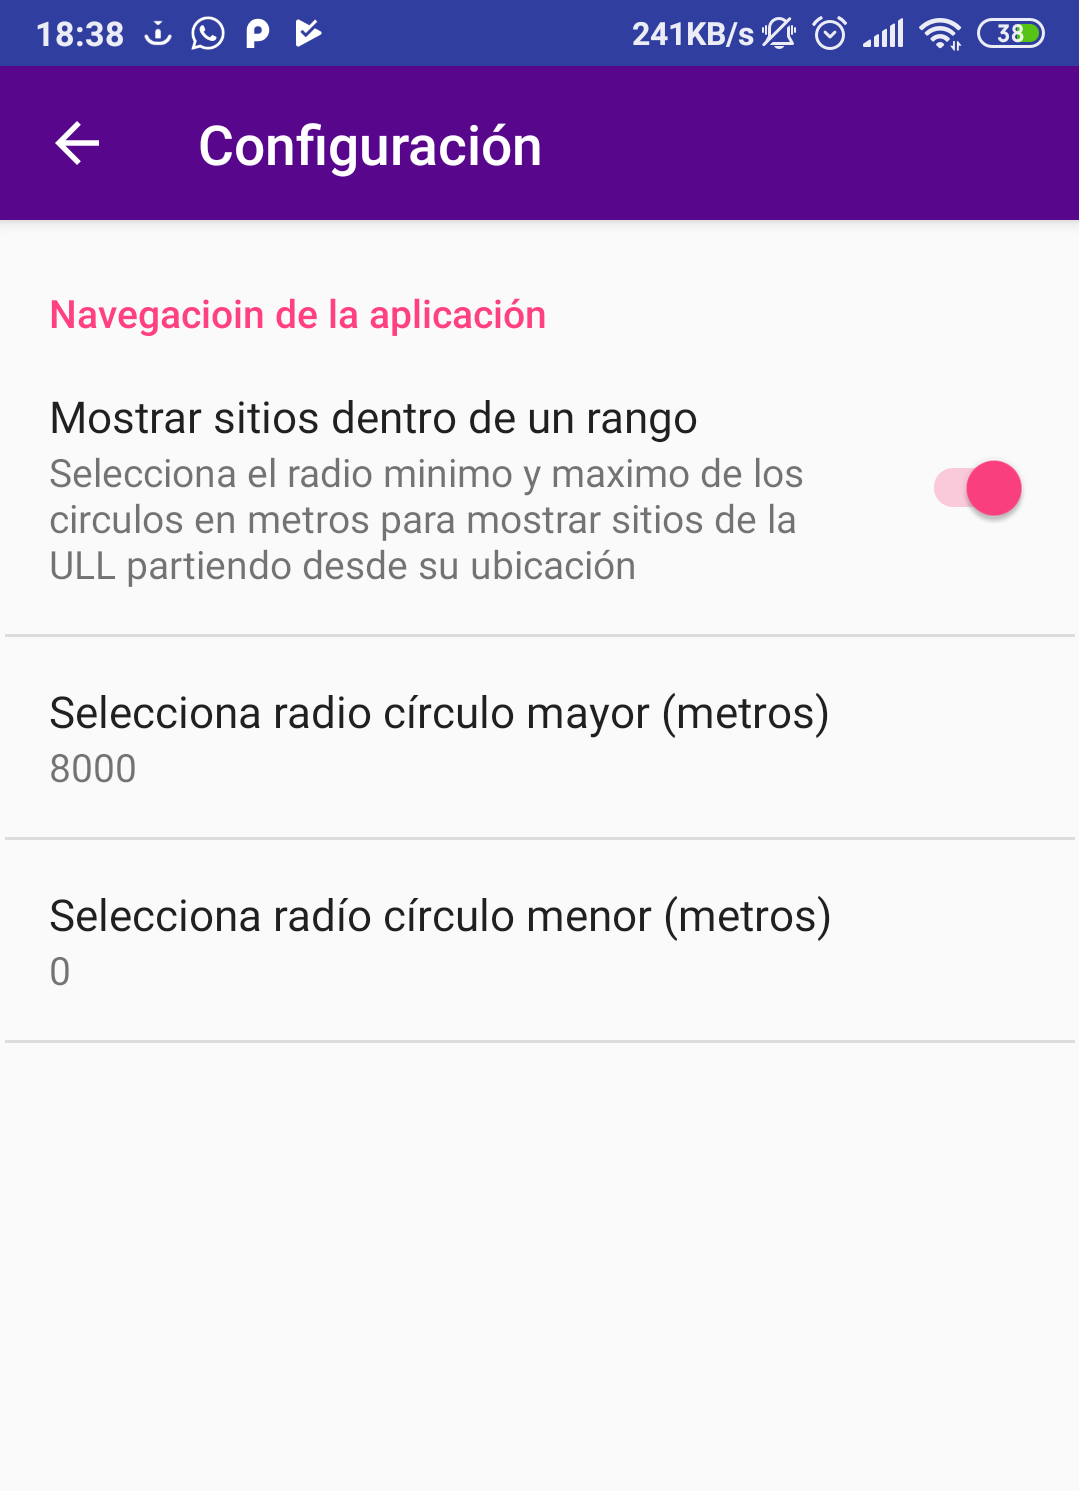
\includegraphics[width=\linewidth]{settingsApp}
    \caption{Configuración.}
    \label{fig:settingsApp}
    \end{subfigure}
    \hfill%
    \begin{subfigure}[h]{0.35\linewidth}
    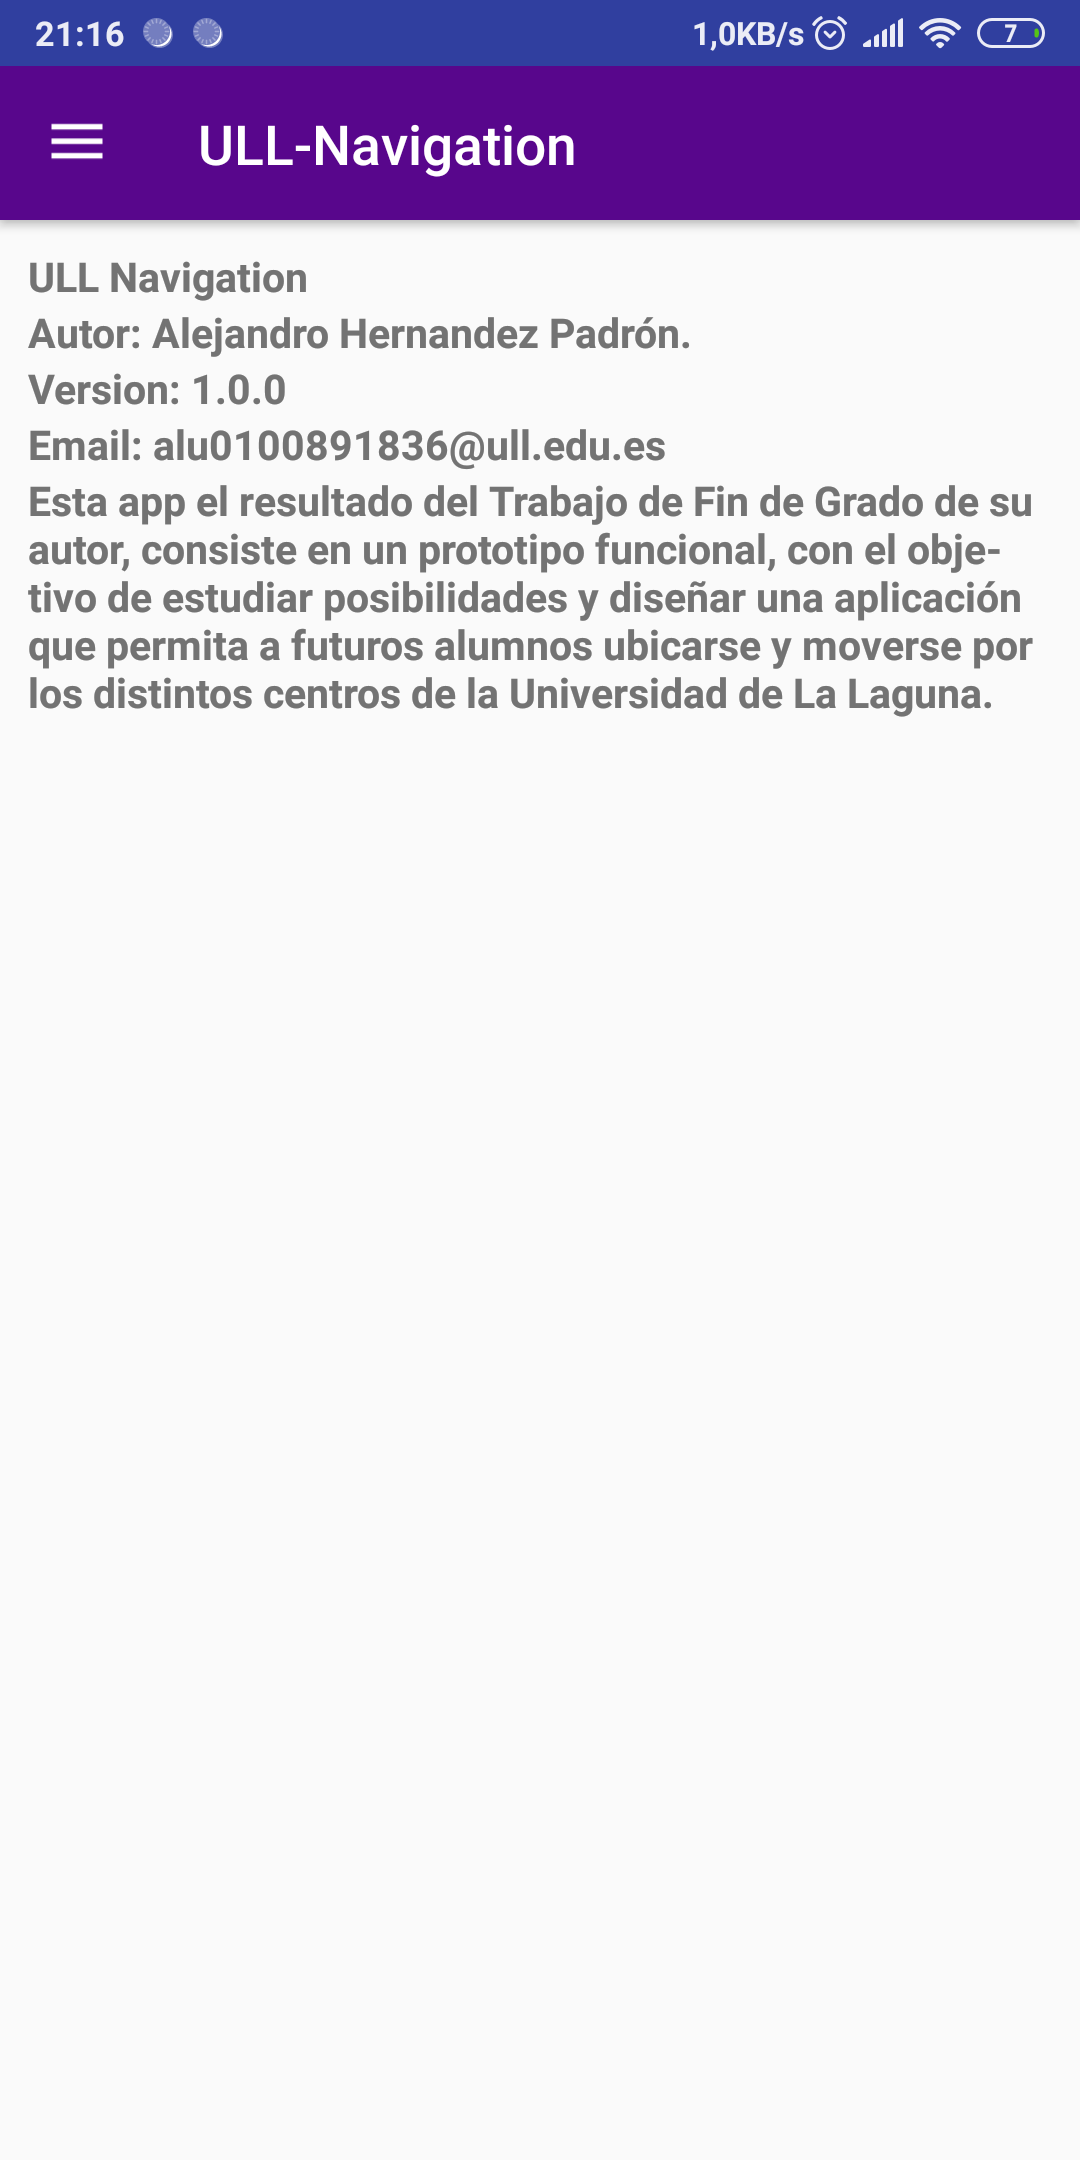
\includegraphics[width=\linewidth]{infoApp}
    \caption{Información.}
    \label{fig:infoApp}
    \end{subfigure}%
    \caption{Ventanas de \textit{Configuración} e \textit{Info} de \textit{ULL-AR}.}
    \hspace*{\fill}%
\end{figure}

\section{Inicio de la aplicación} \label{chap:StartApplication} 

Para comenzar a desarrollar nuestra aplicación, creamos un proyecto nuevo en Android Studio, lo nombramos con el nombre de nuestra aplicación ``ULL-AR" y seguiremos los pasos del IDE para acabar de crear nuestro proyecto. 

Con nuestro proyecto creado, a continuación, explicaremos el funcionamiento e implementación de las primeras ventanas que encontramos cuando iniciamos la aplicación.


\subsection{Ventana inicial}

La primera ventana (véase Figura \ref{fig:splashApp} que aparece en la aplicación es la \textit{Splash Screen}. El objetivo es dar una mejor apariencia a la aplicación y mostrar al usuarios que la aplicación se esta inciando y cargando. 

En esta ventana encontraremos el logotipo de la aplicación en el centro de la pantalla. Este logo se ha diseñado por medio del editor de imagenes online Pixlr \cite{URL::pixlr}. Gracias a este programa hemos podido crear un logotipo simple combinando el icono de la marca de la ULL y el nombre de la aplicación \textit{ULL-AR}.

En un principio la velocidad de carga y transición la siguiente ventana de aplicación se hacia de forma inmediata. Esto se produce por que los recursos necesarios para el inicio de la aplicación son escasos y no tardan en cargarse. Por lo tanto para poder visualizarla correctamente se utilizo un temporizador de tres segundos, para que posteriormente se lance la siguiente ventana, que corresponde a la ventana de \textit{Login}.

Para la implementación de esta ventana hemos indicado en el archivo \textit{AndroidManifest.xml} (Este fichero proporciona información esencial sobre tu aplicación al sistema Android, información que el sistema debe tener para poder ejecutar el código de la app) la ventana o ``activity'' \cite{URL::activity} que inicia la aplicación (véase Listado \ref{lst:manifestInicio}). En esta ventana se le indica el tema del activity que contendrá el logotipo de la aplicación en el centro de la pantalla.

\begin{lstlisting}[language=XML,caption={Fichero \textit{AndroidManifest.xml}, activity que inicia la aplicación.}, label={lst:manifestInicio}]
    ...
    <activity
        android:name=".Activities.SplashActivity"
        android:theme="@style/SplashScreen">
        <intent-filter> 
            <action android:name="android.intent.action.MAIN" />
            <category android:name="android.intent.category.LAUNCHER" />
        </intent-filter>
    </activity>
    ...
\end{lstlisting}

Al mismo tiempo en el archivo \textit{styles.xml} (véase Listado \ref{lst:styleSplash}) indicamos el archivo \textit{splash\_ull.xml} (véase Listado \ref{lst:splashull}) que se encargara de colocar el color del fondo y el logotipo de la aplicación. 

\begin{lstlisting}[language=XML,caption={Fichero \textit{styles.xml}, estilo de la \textit{Splash Screen}.}, label={lst:styleSplash}]
    ...
    <style name="SplashScreen" parent="Theme.AppCompat.NoActionBar">
      <item name="android:windowBackground">@drawable/splash_ull</item>
    </style>
    ...
\end{lstlisting}

\begin{lstlisting}[language=XML,caption={Fichero  \textit{splash\_ull.xml}, xml con el color de fondo y el logotipo de la aplicación. }, label={lst:splashull}]
<layer-list xmlns:android="http://schemas.android.com/apk/res/android">
    <item android:drawable="@color/colorULL"/>
    <item>
        <bitmap
            android:src="@drawable/splash_icon"
            android:gravity="center"/>
    </item>
</layer-list>
\end{lstlisting}

\subsection{Ventana de \textit{Login} }

Esta es la ventana que nos permitira loguearnos con nuestro correo institucional de la ULL (véase Figura \ref{fig:loginApp}). Para ello, dado que la cuentas de la ULL son cuentas de Google, se ha utilizado la API de Google para poder entrar con nuestro correo universitario de forma sencilla y segura.

\subsubsection{ Requisitos }  

Para poder integrar la API de Google necesitaremos integrar los ``Servicios de Google'' en nuestrar aplicación. Para ello hay que entrar en la consola de Firebase \cite{URL::Firebase} y crear un proyecto con el nombre de nuestra aplicación. Una vez dentro de nuestro proyecto, tenemos que indicar que queremos integrar Firebase a un aplicación Android. Posteriormente se nos pedirá el nombre del paquete de nuestra aplicación y la clave ``SHA1". Para obtener esta clave tenenemos que ejecutar en la consola de Android Studio el siguiente comando: 
 
\begin{lstlisting}[ caption={Comando que obtiene la clave SHA1}, label={lst:SHA1}]
    $ keytool -list -v -alias androiddebugkey -keystore ~/.android/debug.keystore
\end{lstlisting} 

Con el nombre del paquete y la clave SHA1, se nos descargará un fichero  con la configuración de los Servicios de Google llamado \textit{google-services.json}. Este fichero hay que colocarlo en la carpeta \textit{app/} de nuestro proyecto.
 
Por ultimo para poder utilizar los Servicios de Google en la aplicación, tenemos que añadir una linea de configuración al fichero \textit{build.gradle} del proyecto en las dependencias (véase Listado \ref{lst:googleSd}) y añadir dos lineas al fichero \textit{build.gradle} de la aplicación (véase Listado \ref{lst:googlepluggin}).

\begin{lstlisting}[caption={Fichero \textit{build.gradle} del proyecto, dependencias para utilizar los Servicios de Google.}, label={lst:googleSd}]
...
buildscript{
    dependencies {
        //Dependencias de los Servicios de Google
        classpath 'com.google.gms:google-services:4.0.0'
    }   
} 
...
\end{lstlisting}
 
\begin{lstlisting}[caption={Fichero \textit{build.gradle} de la aplicación, dependencias y plugin para utilizar los Servicios de Google}, label={lst:googlepluggin}]
...
dependencies {
    //Dependencia necesaria para poder loguearnos con una cuenta de Google
    implementation 'com.google.android.gms:play-services-auth:15.0.1'
}
//Plugin de los Servicios de Google
apply plugin: 'com.google.gms.google-services'
\end{lstlisting}

\subsubsection{ Implementación }

Con todos los requisitos y dependecias ya configuradas en nuestra aplicación, empezaremos a implementar nuestra ventana. Creamos un nuevo activity y lo llamaremos \textit{LoginActivityULL}. Esto nos generará un fichero \textit{LoginActivityULL.java} que tendrá asociado fichero \textit{login\_ull\_activity.xml} con un layout \cite{URL::layout}. Este layout será la vista del activity, con el logotipo de la aplicación y un botón para realizar el login con Google. En el fichero Java se encargará de conectarse con los Servicios de Google para que nos podamos loguear con una cuenta de correo de la ULL.
\bigskip
\bigskip
\lstinputlisting[language=java, caption={Fichero \textit{LoginActivityULL.java}. Código que se encarga de realizar el login del usuario.}, label={code:loginUll.java},]{listings/LoginActivityULL.java} %% LISTING
 
En el Listado \ref{code:loginUll.java} tenemos todos los métodos y conexiones de la API de Google para poder loguearnos. Cuando se presione el botón ``Autentifícate con tu cuenta de la Universidad'' se abrirá un cuadro de dialogo de la API de Google que nos permitirá seleccionar la cuenta con la que deseemos entrar en la aplicación. En caso de que la cuenta no pertenezca a la ULL, es decir, una cuenta que no tenga el formato del dominio de las cuentas de correo de la ULL terminadas en ``@ull.edu.es'', se hará un ``logout'' de la cuenta erronéa y se mostrará un mensaje con el tipo de cuenta necesaria para utilizar la aplicación.

 
 
\section{Modo de Realidad Aumentada}

La técnica de realidad aumentada que se ha implementado en la aplicación, es la de realidad aumentada basada en geolocalización. Es decir, a partir de la ubicación y la orientación del dispositivo, mostramos la información correspondiente de la aplicación superpuesta a la visión de la cámara. Con la orientación, nuestra ubicación y las ubicaciones de las instalaciones de la ULL, podremos hacer los cálculos para identificar a la instalación a la que apuntamos con la cámara del dispositivo.


El fichero \textit{ARNavigation.java} será el activity principal encargado de: la recogida de los datos de los sensores, conexión con el servidor de la aplicación, manejo de los objetos requeridos para la identificación de las instalaciones y de la visualización de la técnica de realidad aumentada implementada.

\subsection{Acceso a los sensores}

Por lo tanto, para implementarla en android vamos que tener acceso a los sensores del dispositivo móvil, como son: el GPS, accelerometro y magnetómetro. 


Para obtener acceso al GPS, vamos a tener que añadir el nuestro \textit{AndroidManifest.xml} los permisos que necesarios para utilizarlo (véase Listado \ref{lst:permisionL}) y, a su vez, preguntar al usuario si nos da permiso para utilizarlo (véase Listado \ref{lst:gpsP}).

\begin{lstlisting}[caption={Fichero \textit{AndroidManifest.xml} del proyecto, permisos para acceder a la ubicación del dispositivo.}, label={lst:permisionL}]
    <uses-permission android:name="android.permission.ACCESS_COARSE_LOCATION" />
    <uses-feature android:name="android.permission.LOCATION_HARDWARE" />
    <uses-permission android:name="android.permission.ACCESS_FINE_LOCATION" />
\end{lstlisting}

\begin{lstlisting}[caption={Código para que el usuario nos conceda permiso para acceder a la ubicacion del dispositivo.}, label={lst:gpsP}]
    if (ContextCompat.checkSelfPermission(this, Manifest.permission.ACCESS_FINE_LOCATION)
        != PackageManager.PERMISSION_GRANTED) {
        requestPermissions(new String[]{Manifest.permission.ACCESS_FINE_LOCATION},                  MY_PERMISSIONS_REQUEST_LOCATION);   
    }
\end{lstlisting}

Con los permisos concedidos, nos bastará con el código mostrado en el Listado \ref{lst:activarL} para empezar a requerir los datos del GPS.

\begin{lstlisting}[caption={Código para activar el GPS del dispositivo.}, label={lst:activarL}]
    locationManager = (LocationManager) getContext().getSystemService(Context.LOCATION_SERVICE);
    locationManager.requestLocationUpdates(LocationManager.GPS_PROVIDER, 3000, 5, this);
    locationManager.requestLocationUpdates(LocationManager.NETWORK_PROVIDER, 3000, 5, this);
\end{lstlisting}

Para acceder a la ultima coordenada registrada por el GPS y así poder ubicar al usuario en el mundo utilizaremos la siguiente linea código:

\begin{lstlisting}[caption={Código para acceder a la última ubicación registrada del GPS.}, label={lst:ubicacionL}]
    currentLocation = locationManager.getLastKnownLocation(LocationManager.GPS_PROVIDER);
\end{lstlisting}


Ahora que tenemos todo los necesario para poder utilizar el GPS del dispositivo, necesitamos conocer la orientación del dispositivo. Para ello hacemos uso de la matriz de rotación que Android calcula a partir del acelorómetro y el magnetómetro. Con esta matriz calcularemos el valor de la brújula magnética del dispositivo, este valor será el que utilizaremos para identificar hacía donde esta orientado el dispositivo en el mundo.


\begin{lstlisting}[caption={Código para acceder a la última ubicación registrada del GPS.}, label={lst:ubicacionL}]
    //Accedemos a los sensores del dispositivo
    mSensorManager = (SensorManager) getSystemService(Context.SENSOR_SERVICE); 
    //Accedemos al calculo de la matriz de rotacion que nos proporciona el valor de la brujula magnetica del dispositivo
    Sensor compass = mSensorManager.getDefaultSensor(Sensor.TYPE_ORIENTATION);
    //Escuchamos a los cambios del sensor
    mSensorManager.registerListener(this, compass, SensorManager.SENSOR_DELAY_NORMAL);    
\end{lstlisting}


Para reconocer la instalaciones que tenemos en frente, escucharemos los cambios del nuestra brújula o ``compass'' para actualizar la nueva orientación y realizar los cálculos que nos permiten identificar las instalaciones, que explicaremos a continuación.


Un dispositivo Android dispone de 3 ejes: x, y, z. Estos ejes se disponen como en la Figura \ref{fig:xyz}. La variable ``compass'' esta formada por un array de tres valores. El primero es denominado acimut y se refiere al ángulo de la orientación sobre la superficie de una esfera. Este valor representa el angulo entre el eje ``y'' del dispositivo y el norte magnético en grados. Cuando miramos el norte el valor del ángulo es 0, al sur es 180º, al este es 90º y al oeste 270º. Para poder trabajar con estos valores lo convertiremos a radianes.  El rango de valores es desde $0$ a $2\pi$


\begin{lstlisting}[caption={Código que se ejecuta cada vez que se registra un cambio en el sensor que calcula la orientacion.}, label={lst:orientacionL}]
    //Escuchamos los cambios en el sensor y hacemos los calculos
    public void onSensorChanged(SensorEvent event) {
        //Valor del sensor en grados
        double radians = event.values[0]; 
        //Convertimos en radianes
        radians = Math.toRadians(radians);
        //Obtenemos la ultima posicion registrada del GPS
        LatLng lastPosition = getCurrentPos();
        if (auxpos != null) { //Si la posicion no es nula
            //Le preguntamos a objeto de la clase ``Navigation'' las instalaciones que se encuentran
            //en esa direccion
            allResultsSites = navULL.whatCanSee(lastPosition, radians);
        }
        //Si obtenemos al menos un resultado
        if (allResultsSites != null) {
            //Obtenemos la instalacion mas cercana, el indice 0 corresponde a la mas cercana
            nearSiteResult = allResultsSites.get(0);
            ... //Mostramos su informacion por pantalla para que usuario sepa que la instalacion  
                //que se encuentra apuntando
            if(allResultsSites.size() > 2) {
                ... //Si obtenemos mas de una instalacion mostramos al usuario el boton
                    //que indica el numero de instalaciones que se encuentran en la misma
                    //direccion 
            }
        } else { ... }
    } 
\end{lstlisting}

\begin{figure}[h]
    \centering
    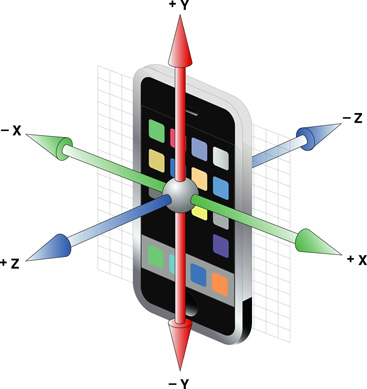
\includegraphics[width=0.4\linewidth]{xyz}
    \caption{Disposición de los ejes de un dispositivo Android.}
    \label{fig:xyz}
\end{figure}    

\subsection{Modelos encargados de la navegación}

\subsubsection{ULLSite.java}

Cada instalacion de ULL se obtiene de una base de datos en formato JSON. Una instalacion tiene una clase asociada que contiene toda su información y los atributos y funciones necesarias para poder trabajar con ella (véase Listado \ref{lst:ULLSite}). Esta clase se construira a partir objeto JSON de cada instalación con el formato de la Figura  \ref{fig:ull-site}.

\lstinputlisting[language=java, caption={Fichero \textit{BaseActivity.java}. Código que se encarga de configurar la vista del Navigation Drawer.}, label={lst:ULLSite},]{listings/models/ULLSite.java}


\begin{figure}[h] 
    \centering
    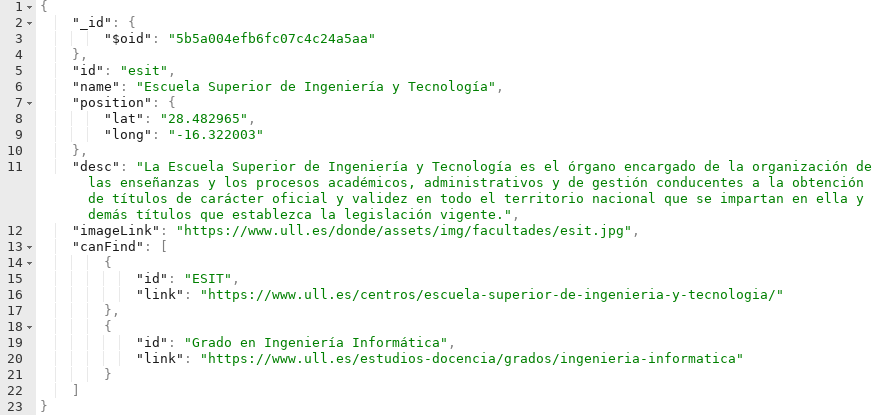
\includegraphics[width=160mm,scale=1]{ull-site}
    \caption{Ejemplo de una instalación de la ULL en la base de datos.}
    \label{fig:ull-site}
\end{figure}


En la clase ULLSite.java encontramos sus atributos con la información general. Los tres útlimos atributos declarados son: ``coneValue'', ``distToSite'' y ``dirToSite''. Estos nos permitirán junto con el objeto ``Vector2D'', que contiene la ubicacion en un plano coordenadas de dos dimensiones (``x'' e ``y''), realizar los cálculos para identificar si nos encontramos en frente de esa instalación o no. La variable ``coneValue'' será un cono formado por la ubicación del dispositivo y la dirección en la que se encuentra la instalación. Este cono determinará el rango a partir del cual se considerará que el dispositivo esta apuntando a la instalación. En la Figura \ref{fig:dirSite} se explica la utilidad de estas variables.

\begin{figure}[h] 
    \centering
    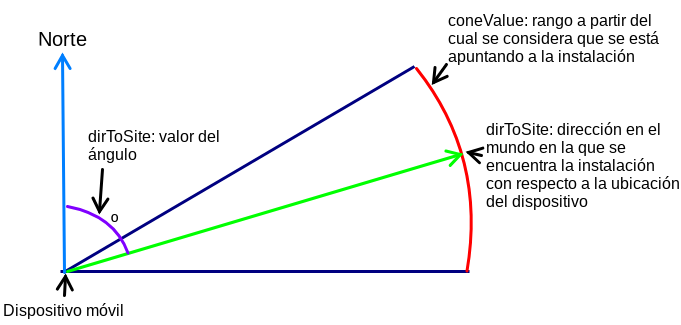
\includegraphics[width=160mm,scale=1]{calculateDirSite}
    \caption{Explicación de las variables ``coneValue'' y ``dirToSite''.}
    \label{fig:dirSite}
\end{figure}

  
\subsubsection{Navigation.java}

La clase ``Navigation'' es la encargada de realizar todos los cáculos para reconocer las instalaciones. A partir de los datos obtenidos de los sensores y de las ubicaciones de las instalaciones permite identificar el centro más cercano que se encuentra en la dirección del dispositivo y también el resto de centros en esta misma dirección. En el Listado \ref{lst:NavigationResumen} podemos ver las variables y métodos de la clase.

\lstinputlisting[language=java, caption={Fichero \textit{Navigation.java}. Clase ``Navigation'' que contiene las variables y métodos para los cálculos de las instalaciones.}, label={lst:NavigationResumen},]{listings/NavigationResumen.java}

A continuación expondremos el funcionamiento de los métodos mas importantes de esta clase:

\begin{lstlisting}[caption={Código para calcular el \textit{coneValue} de identificación de cada instalación.}, label={lst:calculateCone}]
    public double calculateCone(double dist) {
        //Si es una instalacion "cercana" del dispositivo
        if (dist <= NEAR_VALUE){
            //Calculamos el valor del coneValue restandole al valor maximo las distancia a la instalacion por la constante SCALE_CONE_NEAR que permite que esta se escale gradualmente.
            return MAX_CONE_GRADS_NEAR - dist * SCALE_CONE_NEAR;
        }else { //Si es "lejana"
            //Calculamos el valor del coneValue restandole al valor maximo las distancia a la instalacion por la constante SCALE_CONE_FAR que permite que esta se escale gradualmente en instalaciones lejanas.
            double auxCone = MAX_CONE_GRADS_FAR - dist * SCALE_CONE_FAR;
            if (auxCone < MIN_CONE_GRADS) {
                return MIN_CONE_GRADS;
            } else {
                return auxCone;
            }
        }
    }
\end{lstlisting}
 
En Listado \ref{lst:calculateCone} encontramos el método que calcula el tamaño del \textit{coneValue} de una instalación, este vendrá dado en función si lo consideramos una instalación ``cercano'' o ``lejano'' de la ubicación del dispositivo, ya que más adelante en la sección de Configuración \ref{} veremos la distancia máxima y mínima a la que podemos identificar las instalaciones. 
Necesitamos calcular el valor del \textit{coneValue} de modo que cuanto mas cerca nos encontremos de una instalación, mayor sea el rango con el que poder decidir si estamos delante de ella o no y, por el contrario, que este valor sea menor cuando nos estemos lejos de la instalación. 

\begin{lstlisting}[caption={Metodo principal que realiza el cálculo que permite reconocer las instalaciones en frente al dispositivo móvil.}, label={lst:whatCanSee}]
    //Metodo principal que se encarga identificar las instalaciones en frente del dispositivo
    //Recibe la posicion y orientacion actual del dispositivo
    //Devuelve la lista de instalaciones en esa direccion indicando cual es la mas cercana 
    public ArrayList<ULLSite> whatCanSee(LatLng currentPosAux, double actualDir) {
        currentPos.set(actualPos.longitude, actualPos.latitude); //Posicion actual del dispositivo
        currentDir = actualDir;  //Orientacion del dispositivo
        int id = -1;  //indice de la instalacion mas cercana en frente del dispositivo
        double nearSiteDist = maxDist; //distancia maxima valida para identificar un instalacion
        //Array a devolver con las instalaciones encontradas
        ArrayList<ULLSite> result = new ArrayList<>(); 
        //Calculamos todos los sitios que se encuentran entre maxDist y minDist
        for (int i = 0; i < allSites.size(); i++) {
            double distToSite = getDistanceBetween(currentPos, allSites.get(i).getPoint());
            if ((distToSite < maxDist) && (distToSite > minDist)) {
                destSites.add(allSites.get(i));
            }
        }
        //Para cada los sitio dentro del rango anterior 
        for (int i = 0; i < destSites.size(); i++) {  
            //Calculamos la direccion, distancia y valor del cono de cada instalacion a partir 
            //de la actual ubicacion del dispositivo
            double dirToSite = recalculeAng(currentPos.getAngleRad(destSites.get(i).getPoint()));
            double distToSite = getDistanceBetween(currentPos, destSites.get(i).getPoint());
            double coneValue = calculateCone(distToSite);
            //Comprobamos si el dispositivo esta orientado hacia dentro del cono que se forma en  
            //la direccion de la instalacion
            if (isInCone(dirToSite, coneValue)) { 
                //Guardamos los valores calculados anteriormente en el objeto ULLSite del array
                destSites.get(i).setConeValue(coneValue); 
                destSites.get(i).setDirToSite(dirToSite); 
                destSites.get(i).setDistToSite(distToSite); 
                result.add(destSites.get(i)); //Guardamos este sitio como resultado
                if (nearSiteDist > distToSite) { //Comprobamos si es el sitio mas cercano
                    nearSiteDist = distToSite; //Si lo es, actualizamos la distancia mas cercana
                    id = i;                    //Guardamos el indice de la instalacion mas cercana
                }
            }
        }
        if (id != -1) {                        //Si hemos encontrado alguna instalacion
            result.add(0, destSites.get(id));  //La instalacion mas cercana la guadamos la primera
            return result;                     //Devolvemos las instalaciones                   
        } else
            return null;                        //Si no encontramos ninguna instalacion
    }
\end{lstlisting}

El método ``whatCanSee'' \ref{lst:calculateCone} es el función principal que se encarga, partiendo de los datos de ubicación y direccion del dispositivo, de indentificar que instalaciones se encuentran en frente del dispositivo y cual es la más cercana. Para ello. en un primer paso, calculamos las instalaciones que se encuentran a una distancia menor que ``maxDist'' y mayor que ``minDist'' en metros, para reducir la busqueda de las instalaciones la rango generado por esos dos valores. A continuación, para cada instalación anterior calculamos su dirección, posición y el valor del cono, con respecto a la ubicación del dispositivo. Si la instalacion se encuentra orientado dentro del cono que se forma en la dirección de la instalación.

El cálculo del ángulo formado pos dos puntos geográficos lo realizamos con el método ``Vector2D.getAngleRad(Vector2D v2)'' (véase Listado \ref). A este cálculo hay que aplicarles unas transformaciones del ángulo obtenido para que se ajuste a la orientacion del norte magnético como el inicio de la rotación (norte magnético = 0º), para ello el método ``Navigation.recalculeAng(double angleRad)'' se encarga de la correcta reorientación. 

\begin{lstlisting}[caption={Metodo que cálcula el ángulo formado por dos puntos.}, label={lst:whatCanSee}]
    public double getAngleRad(Vector2D v2) {
        double dx = v2.getX() - getX(); //Caculamos las distancias en eje x e y
        double dy = v2.getY() - getY();
        double radian = Math.atan2(dy, dx); //Relizamos la arcotangente para calcular el angulo
        return radian; //Devolvemos el resultado
    }
\end{lstlisting}

\begin{lstlisting}[caption={Método que recalcula en ángulo para orientarlo al norte magnética.}, label={lst:whatCanSee}]
    double aux = rotateRad(angleRad); //Rota -pi/2
    aux = invertAng(aux);             //Inviertimos el angulo 
    return aux;                       //Devolvemos el resultado
}   
\end{lstlisting}

 

\subsection{Obtención de la información}

Como hemos comentado anteriormente, toda la información perteneciente a las instalaciones del Universidad de La Laguna estarán en una base de datos, además, para comunicarnos con esta dispondremos de un servidor que antienda a las peticiones de la aplicación y se conecte y nos envié estos datos. Más adelante, en el capítulo \ref{chap:BackEnd}, explicaremos detalladamente como funciona esta base de datos y servidor. Por ahora nos centraremos en explicar como realizamos la conexión con el servidor y el tipo de respuesta que obtenemos.

Para poder realizar una petición al servidor utilizaremos la clase ``GetData'' (véase Listado \ref{lst:getData}). Que formaliza la petición con la url que le pasemos como parámetro la funcion ``doInBackground'' y nos devuelve un string con la respuesta del servidor. 

\lstinputlisting[language=java, caption={Fichero \textit{GetData.java}, Código encargado de la conexión con el servidor y manejar la respuesta.}, label={lst:getData},]{listings/models/GetData.java} 

En el Listado \ref{lst:getSitesFromDB} encontramos el método ejecutado en fichero \textit{ARNavigation.java} para realizar la conexión el servidor para obtener la respuesta de la base de datos con todas las instalaciones de ULL. Para posteriormente crear una instancia de la clase ``Navigation'' con todas las instalaciones de la base de datos en formato JSON. Este objeto lo denominaremos con el nombre de ``navULL'' y será el objeto encargado de identificar las instalaciones y trabajar con ellas.
\begin{lstlisting}[caption={Método que conecta con el servidor y recibe la respuesta con todas las instalaciones de la base de datos.},  label={lst:getSitesFromDB}]
    private void getSitesFromDB() {
        try{
        GetData getSites = new GetData();
        String sites = getSites.execute("https://server-ull-ar.herokuapp.com/api/ull-sites").get();
        JSONArray array = new JSONArray(sites);
        //Creamos una instancia del la clase "Navigation" con todas las instalaciones
        //Este es el objeto encargado de encontrar las instalaciones
        navULL = new Navigation(array); 
        } catch (JSONException e) {...}
}
\end{lstlisting}

Los últimos datos que necesitamos para nuestro trabajar en el objeto ``navULL'' son los valores de ``maxRadius'' y ``minRadius'', que podemos editar en la ventana de \textit{Configuración} y que podemos acceder desde cualquier activity (véase Listado \ref{lst:shared}) gracias a las ``Shared Preferences". Las Shared Preferences son un conjunto de datos accesible desde cualquier clase de la aplicación y que se utiliza para guardar los ajustes del usuario.

\begin{lstlisting}[language=java, caption={Ficher \textit{ARNavigation.java}, Código que se encarga de guardar los valores de ``maxDist'' y ``minDist'' del objeto ``navULL''},  label={lst:shared}]
    private void getRadius() {
        try {
            //Obtenemos los valores configurables "maxRadius" y "minRadius" en la ventana de "Configuracion"
            settingsPref = PreferenceManager.getDefaultSharedPreferences(getContext());
            String auxMaxRadius = settingsPref.getString("maxRadius", "null");
            String auxMinRadius = settingsPref.getString("minRadius", "null");
            navULL.setMaxDist(Integer.parseInt(auxMaxRadius)); //Guradamos el valor "maxRadius"
            navULL.setMinDist(Integer.parseInt(auxMinRadius)); //Guradamos el valor "minRadius"
        }catch (Exception e){ ... }
    }
\end{lstlisting}


\subsection{Visualización}

Para la visualización de la técnice de realidad aumentada por geolozación, se utiliza el activity ``ARNavigation''
como ventana que mostrará el contenido. Esta activity hereda de la clase ``ARActivity'' perteneciente al  SDK de Kudan para Android Studio. Este SDK nos permite el reconocimiento de objetos e imágenes a trávez de la camara del dispositivo y queda como recurso para una futura ampliación de la funcionalidad de la aplicación. El uso principal de esta clase es el acceso que otorga a cámara del dispositivo como vista del activity. Es decir, nos permite visualizar en la ventana lo que esta observando la cámara.

Para poder hacer uso del SDK de Kudan tenemos que descargarnos el SDK y configurar la ``ARAPIkey'' específica para nuestro proyecto. Ambos los podemos encontrar en la página oficial de Kudan \cite{URL::kudan}. 

El que contiene el SDK descargado, llamado \textit{KudaAR.aar}, tenemos que pegarlo en la carpeta \textit{/app/libs/} de nuestro proyecto. A continuación tenemos de añadir la siguiente linea de código a las dependencias del fichero \textit{build.gradle} de la aplicación:

\begin{lstlisting}
    implementation(name: 'KudanAR', ext: 'aar')
\end{lstlisting}

La configuración de la clave de la API de Kudan se realizará con el código del Listado \ref{lst:arapi}.
\begin{lstlisting}[caption={Fichero \textit{ARNavigation.java''}. Código para configurar la API de Kudan.},  label={lst:arapi}]
    protected void onCreate(Bundle savedInstanceState) { //Cuando se inicie el activity
        ...
        ARAPIKey key = ARAPIKey.getInstance(); 
        key.setAPIKey("ARAPIKey..."); //ARAPIKey, clave generada por Kudan para el proyecto
    }
\end{lstlisting}
 
El fichero \textit{aractivity.xml} (véase Listado \ref{lst:aractivity.xml}) contiene el layout con la información a mostrar al usuario cuando esté delante de una instalación. Este layout muestra al usuariom en la parte superior de la ventana, el nombrre de instalación ante la que se encuentra y un botón que le permite ir a la ficha de información de la instalación. Además incorpora un botón en la parte inferior que le indica el número de instalacione adicionales que encuentran en la misma dirección. Al pulsar este botón se despliega una lista estas instalaciones.

\lstinputlisting[stringstyle=\color{purple},language=XML, caption={Fichero \textit{aractivity.xml}. Layout del activity ``ARNavigation''.}, label={lst:aractivity.xml},]{listings/aractivity.xml}

Los elementos del layout se mostrarán o ocultarán en función de si nos encontramos en frente de una instalcion o no, como podemos ver en el Listado \ref{lst:orientacionL}, se muestra cuando se alterna la información del layout.

Por último tenemos que configurar el funcionamiento de los botones ``moreInfoButton'' y ``moreSitesButton'' (véase Listado \ref{lst:infobutton}), que mostrarán una ventana con la ficha de información de la instalación (véase Figura \ref{fig:ull-site}) y una ventana con una lista que contiene las instalaciones que tambien se  encuentran la dirección a la que estamos orientados. 



\begin{lstlisting}[caption={Fichero \textit{ARNavigation.java}. Código para manejar los eventos de los botones.},  label={lst:infobutton}]
    public void onClick(View v) {
        if(v.getId() == moreSitesButton.getId()){ //Si coincide
            //Nos preparamos iniciar el activity que muestra la lista de los sitios adicionales
            Intent intent = new Intent(this, SitesListActivity.class);
            ArrayList aux = new ArrayList(moreResultsSites.subList(1, moreResultsSites.size()-1));
            SitesArray sitesArray = new SitesArray(aux);
            //Le pasamos la lista con los sitios a mostrar
            intent.putExtra("sitesToShow", sitesArray);
            startActivity(intent); //Iniciamos el activity
        }
        if(v.getId() == moreInfoButton.getId()){ //Si coincide
            //Nos preparamos iniciar el activity que muestra la descripcion de la instalacion
            Intent intent = new Intent(getApplicationContext(), SiteDescriptionActivity.class);
            ULLSiteSerializable actualULLSite = new ULLSiteSerializable(nearSiteResult);
            //Le pasamos como "extra" el objeto que contiene la informacion del sitio
            intent.putExtra("actualULLSite", actualULLSite);
            startActivity(intent); //Iniciamos el activity
        }
    }
\end{lstlisting}


\section{Fragmentos}

Los fragmentos \cite{URL::fragment} actuan como una sección modular de un activity que tiene su ciclo de vida propio, es decir, recibe sus propios eventos de entrada y que puedes agregar o quitar mientras la actividad se esté ejecutando. Se han utilizados estos fragmentos para mostrar el contenido de ciertas ventanas de la aplicación. La principal ventaja que nos aportan los frangemetos, es la facilidad que se tiene para intercambiar fragmentos dentro de un mismo activity y la mejora de rendimiento que se obtiene con respecto a creación de un activity para cada ventana que queramos en nuestra aplicación.

\subsection{MapsFragment}
       
Este fragmento contiene el mapa generado por la API de Google Maps. Para poder utilizar esta API, desde la onsola de desarrolladores de Google \cite{URL::consoleGoogle}. En ella tenemos que tener nuestro proyecto creado, para después habilitar la API de ``Maps SDK for Android". Una vez habilitada se nos otorgará una clave que tendremos que en el fichero \textit{app/res/values/google\_maps\_api.xml} (véase Listado \ref{lst:apiMaps}).

\begin{lstlisting}[stringstyle=\color{purple},language=XML,caption={Fichero \textit{google\_maps\_api.xml}.},  label={lst:apiMaps}]
<resources>
    <string name="google_maps_key" templateMergeStrategy="preserve" translatable="false">API_Maps</string>
</resources>
\end{lstlisting}
 
A su vez, debemos añadir la siguiente linea a las dependencias de fichero \textit{build.gradle} de la aplicación:
 
\begin{lstlisting}
    implementation 'com.google.android.gms:play-services-maps:15.0.1'
\end{lstlisting}

Con esto ya podremos utilizar la API de Google Maps en nuestra aplicación. Ahora nos toca configurar el nuestro fragmento de que contendrá la vista de Google Maps. 

Crearemos un fragmento en Android Studio con el nombre de \textit{MapsFragment}. Se nos generará un fichero llamado \textit{MapsFragment.java} y un layout asociado, \textit{fragment\_maps.xml}.

La clase del fichero ``MapsFragment'' (véase Listado \ref{lst:mapsF}) se encargará de: obtener la ubicación, dibujar en el mapa los marcadores las instalaciones de ULL, la ubicación del dispositivo y, si se activa en los ajustes, las dos circunferencias, cuyo centro es la ubicacion del dispositivo y que representaran un rango de busqueda de las instalaciones. Este rango funcionará a modo de que solo aparezcan las instalaciones que se encuentran en el espacio entre las dos circunferencias. En esta clase se harán uso de los métodos que ya vimos para obtener la ubicación GPS, las instalaciones de la base de datos y los datos necesarios guardados en las Shared Preferences.   

\bigskip

\lstinputlisting[caption={Fichero \textit{MapsFragment.java}. Métodos principales.}, label={lst:mapsF},]{listings/MapsFragment.java}

El fichero \textit{fragment\_maps.xml}(véase Listado \ref{lst:mapsL}) contiene la vista del mapa de Google Maps en el cual se dibujaran los marcadores y los circulos que hemos comentado. Además incorpora un botón con el nombre de ``AR Mode'' que lanzará la ventana que contiene el modo de realidad aumentada.

\lstinputlisting[stringstyle=\color{purple},language=XML,caption={Fichero \textit{fragment\_maps.xml}.}, label={lst:mapsL},]{listings/fragment_maps.xml}
    

\subsection{HomeFragment}

El fragmento ``HomeFragment'' es la primera vista que encontramos cuando iniciamos con éxito la aplicación. Para el diseño se decidio por utilizar el modelo de ``RecyclerView'' \cite{URL::recycler}. Este modelo nos permite la visualización de listas de elementos o items de una forma más flexible, permitiendo configurar el contenido de cada elemento mediante el uso de adaptadores. Estos adaptadores permiten crear las vistas de los items de una lista a partir del contenido de cada uno de ellos. Además, gestiona los eventos cuando un item es seleccionado.

El contenido de cada item vendrá dada por la clase ``ItemHome'' (véase Listado \ref{lst:itemhom}). Los atributos de esta clase serán: una imagen, un nombre, una variable si indica si es o no un enlace externo del navegador y la url del enlace.

\begin{lstlisting}[caption={Fichero \textit{ItemHome.java}.},  label={lst:itemhom}]
    public class ItemHome {
        private String name;        //Nombre
        private String image;       //Ruta de la imagen
        private boolean isWebLink;  //Si es true es un enlace web externo
        private String link;        //Ruta del enlace
        //Constructor con los parametros
        public ItemHome(String name, String image, boolean isWebLink, String link){
            this.name = name;
            ...
        }
        ... //Get() y Set() metodos de los atributos
    }
\end{lstlisting}

Con una lista de estos items, nuestro adaptor construirá el layout de cada uno de los items y luego se incorporarán a la vista de RecyclerView. La clase encargada de este procedimiento se llamará ``ItemHomeAdapter'' y hereda del adaptador ``RecyclerView.Adapter'' (véase Fichero \ref{lst:adapterItem}). Los atributos de esta clase son: una lista de los items, el layout con el diseño de cada item y un objeto ``OnItemClickListener'', que manejará los eventos de cada item. Dentro de esta clase, tendremos una clase ``ViewHolder'' que hereda de ``RecyclerView.ViewHolder'' y se encargará de enlazar el contenido de cada item con su layout. El layout con la vista de cada item lo encontraremos en el fichero \textit{adapter\_item\_home.xml} (véase Fichero \ref{lst:itemView}). Este layout contendrá la imagen del item en la parte superior y el nombre inferior.
     
\begin{lstlisting}[caption={Fichero \textit{ItemHomeAdapter.java}, clase que contruye las vistas de los items.},  label={lst:adapterItem}]
    public class ItemHomeAdapter extends RecyclerView.Adapter<ItemHomeAdapter.ViewHolder> {
        private List<ItemHome> items;
        private int layout;
        private OnItemClickListener itemClickListener;
        public ItemHomeAdapter(List<ItemHome> items, int layout, OnItemClickListener listener){
            ... //Asignamos a los atributos con sus respectivos valores
        }
        //El parametro @ViewGroup parent contendra la vista de todos los items
        public ViewHolder onCreateViewHolder(@NonNull ViewGroup parent, int viewType) {
            View v = LayoutInflater.from(parent.getContext()).inflate(layout, parent, false);
            ViewHolder vh = new ViewHolder(v);     //Objeto ViewHolder  
            return vh;                             //Devolvemos la vista    
        }
        //Enlazamos cada item con su objeto ViewHolder
        public void onBindViewHolder(@NonNull ViewHolder holder, int position) {
            holder.bind(items.get(position), itemClickListener);
        }
        //Clase que hereda de RecyclerView.ViewHolder que sera la vista de cada item
        public static class ViewHolder extends RecyclerView.ViewHolder { 
            public TextView itemName;     
            public ImageView itemImage;   
            ...
            public ViewHolder(View itemView) { //Constructor con el layout
                ... //Enlazamos los objetos con el layout
                this.itemName= itemView.findViewById(R.id.textView_home_item);     
                this.itemImage = itemView.findViewById(R.id.imageView_home_item);
            }
            //Asignamos a cada vista el contenido de su item correspondiente 
            public void bind(final ItemHome itemHome, final OnItemClickListener listener){
                this.itemName.setText(itemHome.getName()); //Asignamos el texto
                ... //Asingamos la ruta de la imagen
                itemView.setOnClickListener(new View.OnClickListener() { ... });//Listener del item
        }
    }
\end{lstlisting}
    
\lstinputlisting[stringstyle=\color{purple},language=XML,caption={Fichero \textit{adapter\_home\_item.xml}.}, label={lst:itemView},]{listings/adapter_home_item.xml}

La clase ``HomeFragment''(véase Listado \ref{lst:homeF}) se encargará de instanciar los objetos de la clase ``ItemHome'' y el adaptador, ``ItemHomeAdapter'', para que se situén correctamente en la vista que contiene el RecyclerView (véase Listado \ref{lst:homeL}). 
  
\lstinputlisting[caption={Fichero \textit{HomeFragment.java}.}, label={lst:homeF},]{listings/HomeFragment.java}

\lstinputlisting[stringstyle=\color{purple},language=XML,caption={Fichero \textit{fragment\_home.xml}.}, label={lst:homeL},]{listings/fragment_home.xml}



\subsection{AboutFragment}

El fragmeto ``AboutFragment'' se encargar de mostar la ventana de la aplicación con la información general de la aplicación. Este consta simplemente de un fichero \textit{Fragment.java} que muestra el layout que contiene esta información (véase Listado \ref{lst:aboutL}).

\lstinputlisting[stringstyle=\color{purple},language=XML,caption={Fichero \textit{fragment\_about.xml}.}, label={lst:aboutL},]{listings/fragment_about.xml}


\section{Menú}

El menú de la aplicación constituye el elemento principal por el que el usuario navegará por la misma. Por ello se optado por incorporar un menú lateral deslizante llamado \textit{Navigation Drawer}. Este ha sido implementado por Google y lo encontramos en sus principales aplicaciones como ``Gmail'' y ``Google Play''. Un menú Navigation Drawer es un layout que incorpora dentro del mismo la vista de otras ventanas que se encuentren formato de fragmentos  y facilita que el cambio entre los fragmentos sea fluido y rápido. Este menú (véase Figura \ref{fig:menuApp}) se desplegará pulsando en la esquina superior izquierda de la aplicación.
   
El fichero \textit{navigation\_draw.xml} contiene la vista del Navigation Draw. Aqui contamos con layout para el contenido principal a mostrar en la aplicación, la barra superior de la aplicación la que ira el nombre de \textit{ULL-AR}, un ``FrameLayout'' en el que ira el fragmento actual a mostrar y un ``NavigationView'' que será la vista del menú que un inicio estará sin desplegar.

\lstinputlisting[stringstyle=\color{purple},language=XML, caption={Fichero \textit{navigation\_draw.xml}. Layout del Navigation Drawer.}, label={code:navigation_draw.xml},]{listings/navigation_draw.xml}

Para la implementación del menú se utilizado una clase heredable llamada \textit{BaseActivity.java} la cual incorpora la vista del Navigation Drawer, gestionará las opciones de el menú, cambiará los fragmentos y lanzará los activities principales de ULL-AR. 


\lstinputlisting[language=java, caption={Fichero \textit{BaseActivity.java}. Código que se encarga de configurar la vista del Navigation Drawer.}, label={BaseActivity.java},]{listings/BaseActivity.java}


En cuanto al menú del Navigation Drawer, tenemos una cabecera (véase Listado \ref{code:header_navigation_drawer.xml}) con una imagen de la ULL y el debajo el nombre del usuario. Debajo de la cabecera tenemos las opciones del menú que vienen dadas por el fichero \textit{nav\_options.xml} (véase Listado \ref{lst:nav_options.xml}). Cada uno de los items de opciones tiene un id, icono asociado y nombre.


\lstinputlisting[stringstyle=\color{purple},language=XML, caption={Fichero \textit{header\_navigation\_drawer.xml}. Cabecera del Navigation Drawer.}, label={code:header_navigation_drawer.xml},]{listings/header_navigation_drawer.xml}
   

\lstinputlisting[stringstyle=\color{purple},language=XML, caption={Fichero \textit{nav\_options.xml}. Opciones del menu Navigation Drawer.}, label={lst:nav_options.xml},]{listings/nav_options.xml}
        
\section{Instalaciones}

En la base de datos nos encontramos con la gran mayoría de las instalaciones de la ULL. Recordamos que todas estas instalaciones constan de su nombre, posicion, una breve descripción del mismo y una lista de enlaces a los servicios, grados, departamentos, etc. Toda esta información es accesible por el usuario, mediante la ventana de \textit{Todas las instalaciones} (véase Figura \ref{fig:allSitesApp}). Esta ventana permite al usuario buscar la facultad, edificio o centro, que se encuentre en la base de datos, para posteriormente permitirle acceder a la ficha de información de la instalación (véase Figura \ref{fig:siteInfoApp}). En esta ficha se encontrará el resto de la información con respecto a es instalación.

En la ventana de \textit{Todas las instalaciones} nos aparecerá una lista con todas las instalaciones con: su imagen a la izquierda y su nombre y descripción a la derecha. Para la creación de los items de la lista se opto por el uso de adaptadores al igual que en el fragmento ``HomeFragment'', pero sin la necesidad de una vista RecyclerView. La clase encargada de representar las instalaciones es ``SiteAdapter'', la cual hereda de la clase ``BaseAdapter'' de Android y, además, implementa la interfaz ``Filterable'' que permite aplicar, de forma dinámica, un filtro de busqueda sobre la lista de las instalaciones (véase Listado \ref{lst:SiteAdapter.java}). 



\lstinputlisting[language=java, caption={Fichero \textit{SiteAdapter.java}.}, label={lst:SiteAdapter.java},]{listings/adapters/SiteAdapter.java}

Para la lista con los objetos a representar, se ha utilizado la clase ``ULLSiteSerializable'' que es una copia la clase  ``ULLSite'' (véase Listado \ref{lst:ULLSite}) pero que implementa la interfaz ``Serializable'' para permitir el paso de este objeto entre activities. 

El activity ``SiteListActivity'' se encargará de instanciar el adaptador con la lista de instalaciones que reciba del anterior activity y, dispondrá en la barra superior de la aplicación la barra de busqueda. Esta barra de busqueda le dirá al adaptador el filtro que tiene aplicar cada vez que se escriba en ella o cuando el usuario le de al botón de buscar. Cuando una instalación de la lista sea seleccionada se lanzará el activity ``SiteDescriptionActivity'' y se le pasará el objeto que contiene la instalación seleccionada.

\lstinputlisting[language=java, caption={Fichero \textit{SiteListActivity.java}.}, label={lst:SiteListActivity.java},]{listings/SitesListActivity.java}
    

La activity ``SiteDescriptionActivity'' muestra toda la información de la instalación contenida en el objeto ``ULLSiteSerializable'' que envió activity que lo ejecuto o lanzo a este. Es una ventana que dispondrá: de la imagen de la instalación junto con botón en la parte inferior que abrirá la ruta de la aplicación en Google Maps, el nombre de la instalación, su descripción y una serie de enlaces relacionados con esta. Cuando uno de los enlaces es seleccionado, se abrirá el navegador externo del dispositivo móvil.

 
\lstinputlisting[language=java, caption={Fichero \textit{SiteListActivity.java}.}, label={lst:SiteListActivity.java},]{listings/SiteDescriptionActivity.java}
 
    
\section{Preferencias del usuario}

Necitamos un lugar donde el usuario pudiera editar los ajustes de la aplicación. Se ha utilizado la clase ``PrefenceActivity'' que nos ofrece Android para diseñar la ventana. El fichero \textit{pref\_nav\_setting.xml} (véase Listado \ref{lst:pref_nav_setting.xml} contendrá la lista con los ajustes. Estos ajustes nos permitiran decidir si queremos encontrar las instalaciones, en el mapa o en el modo realidad aumentada, dentros de dos circunferencias y la dimensiones en metros de ambos radios. 

\lstinputlisting[language=XML, caption={Fichero \textit{pref\_nav\_setting.xml}.}, label={lst:pref_nav_setting.xml},]{listings/pref_nav_settings.xml}

Esta ventana de preferencias que nos ofrece Android nos permite trabajar con las Shared Preferences para guardar los ajustes y poder acceder a ellos en otras ventanas de la aplicación. En la clase ``SettingsULLActivity'' insertamos la vista con nuestras preferencias.

\lstinputlisting[float,floatplacement=H,language=java, caption={Fichero \textit{SettingsULLActivity.java}.}, label={lst:SettingsULLActivity.java},]{listings/SettingsULLActivity.java}
